\subsection{Application}
The Application is composed of two different sub-components (Figure
\ref{fig:sd-app-init}):

\begin{itemize}
  \item \textbf{Application Logic Layer}: handles the application logic
    (slightly abusing the notation, we will often refer to it simply as
    \textit{Application Layer});
  \item \textbf{Interface Layer (IL)}: provides the remote services to Application
    Layer by acting as an interface towards the underlying middleware layer.
\end{itemize}

\subsubsection{Application Layer}\label{sec:sol-des-app-layer}

\paragraph{Types of entities}
Three types of entities have been identified
\begin{itemize}
  \item \textit{Active}: an entity capable to start an action by itself,
  providing it the computational resources it needs;
  \item \textit{Reactive}: an entity with an inner state, that only acts on
reaction to external inputs, and it is not capable to start an action by itself;
  \item \textit{Passive}: an entity with an internal state (if necessary) which
is immutable. As a Reactive entity it only acts on reaction to external inputs,
and it is not capable to start an action by itself.
\end{itemize}
\begin{table}[H]
\centering
\begin{tabular}{|l|l|}
\hline
\rowcolor{BlueGreen}
Type     & Entities                                 \\ \hline
Active   & pedestrian, bicycle, motorcycle, car, bus, traffic light \\ \hline
Reactive & road, crossroads, sidewalk, bike lane, crossing, house \\ \hline
Passive  & road signs                               \\ \hline
\end{tabular}
\caption{Types of entities}
\label{tab:entity_type}
\end{table}
Entity types have the following dependencies:
\begin{itemize}
  \item \textit{Active} entities provides inputs to the \textit{Reactive}
entities (solid line);
  \item \textit{Active} and \textit{Reactive} entities can use \textit{Passive}
entities, the dependency is not strict (dashed line).
\end{itemize}
\begin{figure}[H]
  \centering
  \includegraphics[width=.35\columnwidth]{images/solution/entity_type_dependency.eps}
  \caption{Dependencies between entity types}
  \label{fig:sd-entity-types-deps}
\end{figure}




Figure \ref{fig:sd-app-backend-architecture} provides an architectural overview
of the main classes which compose the application layer.
As shown in the figure, the core packages have been named according to
Table \ref{tab:entity_type}.

\begin{figure}[H]
  \centering
  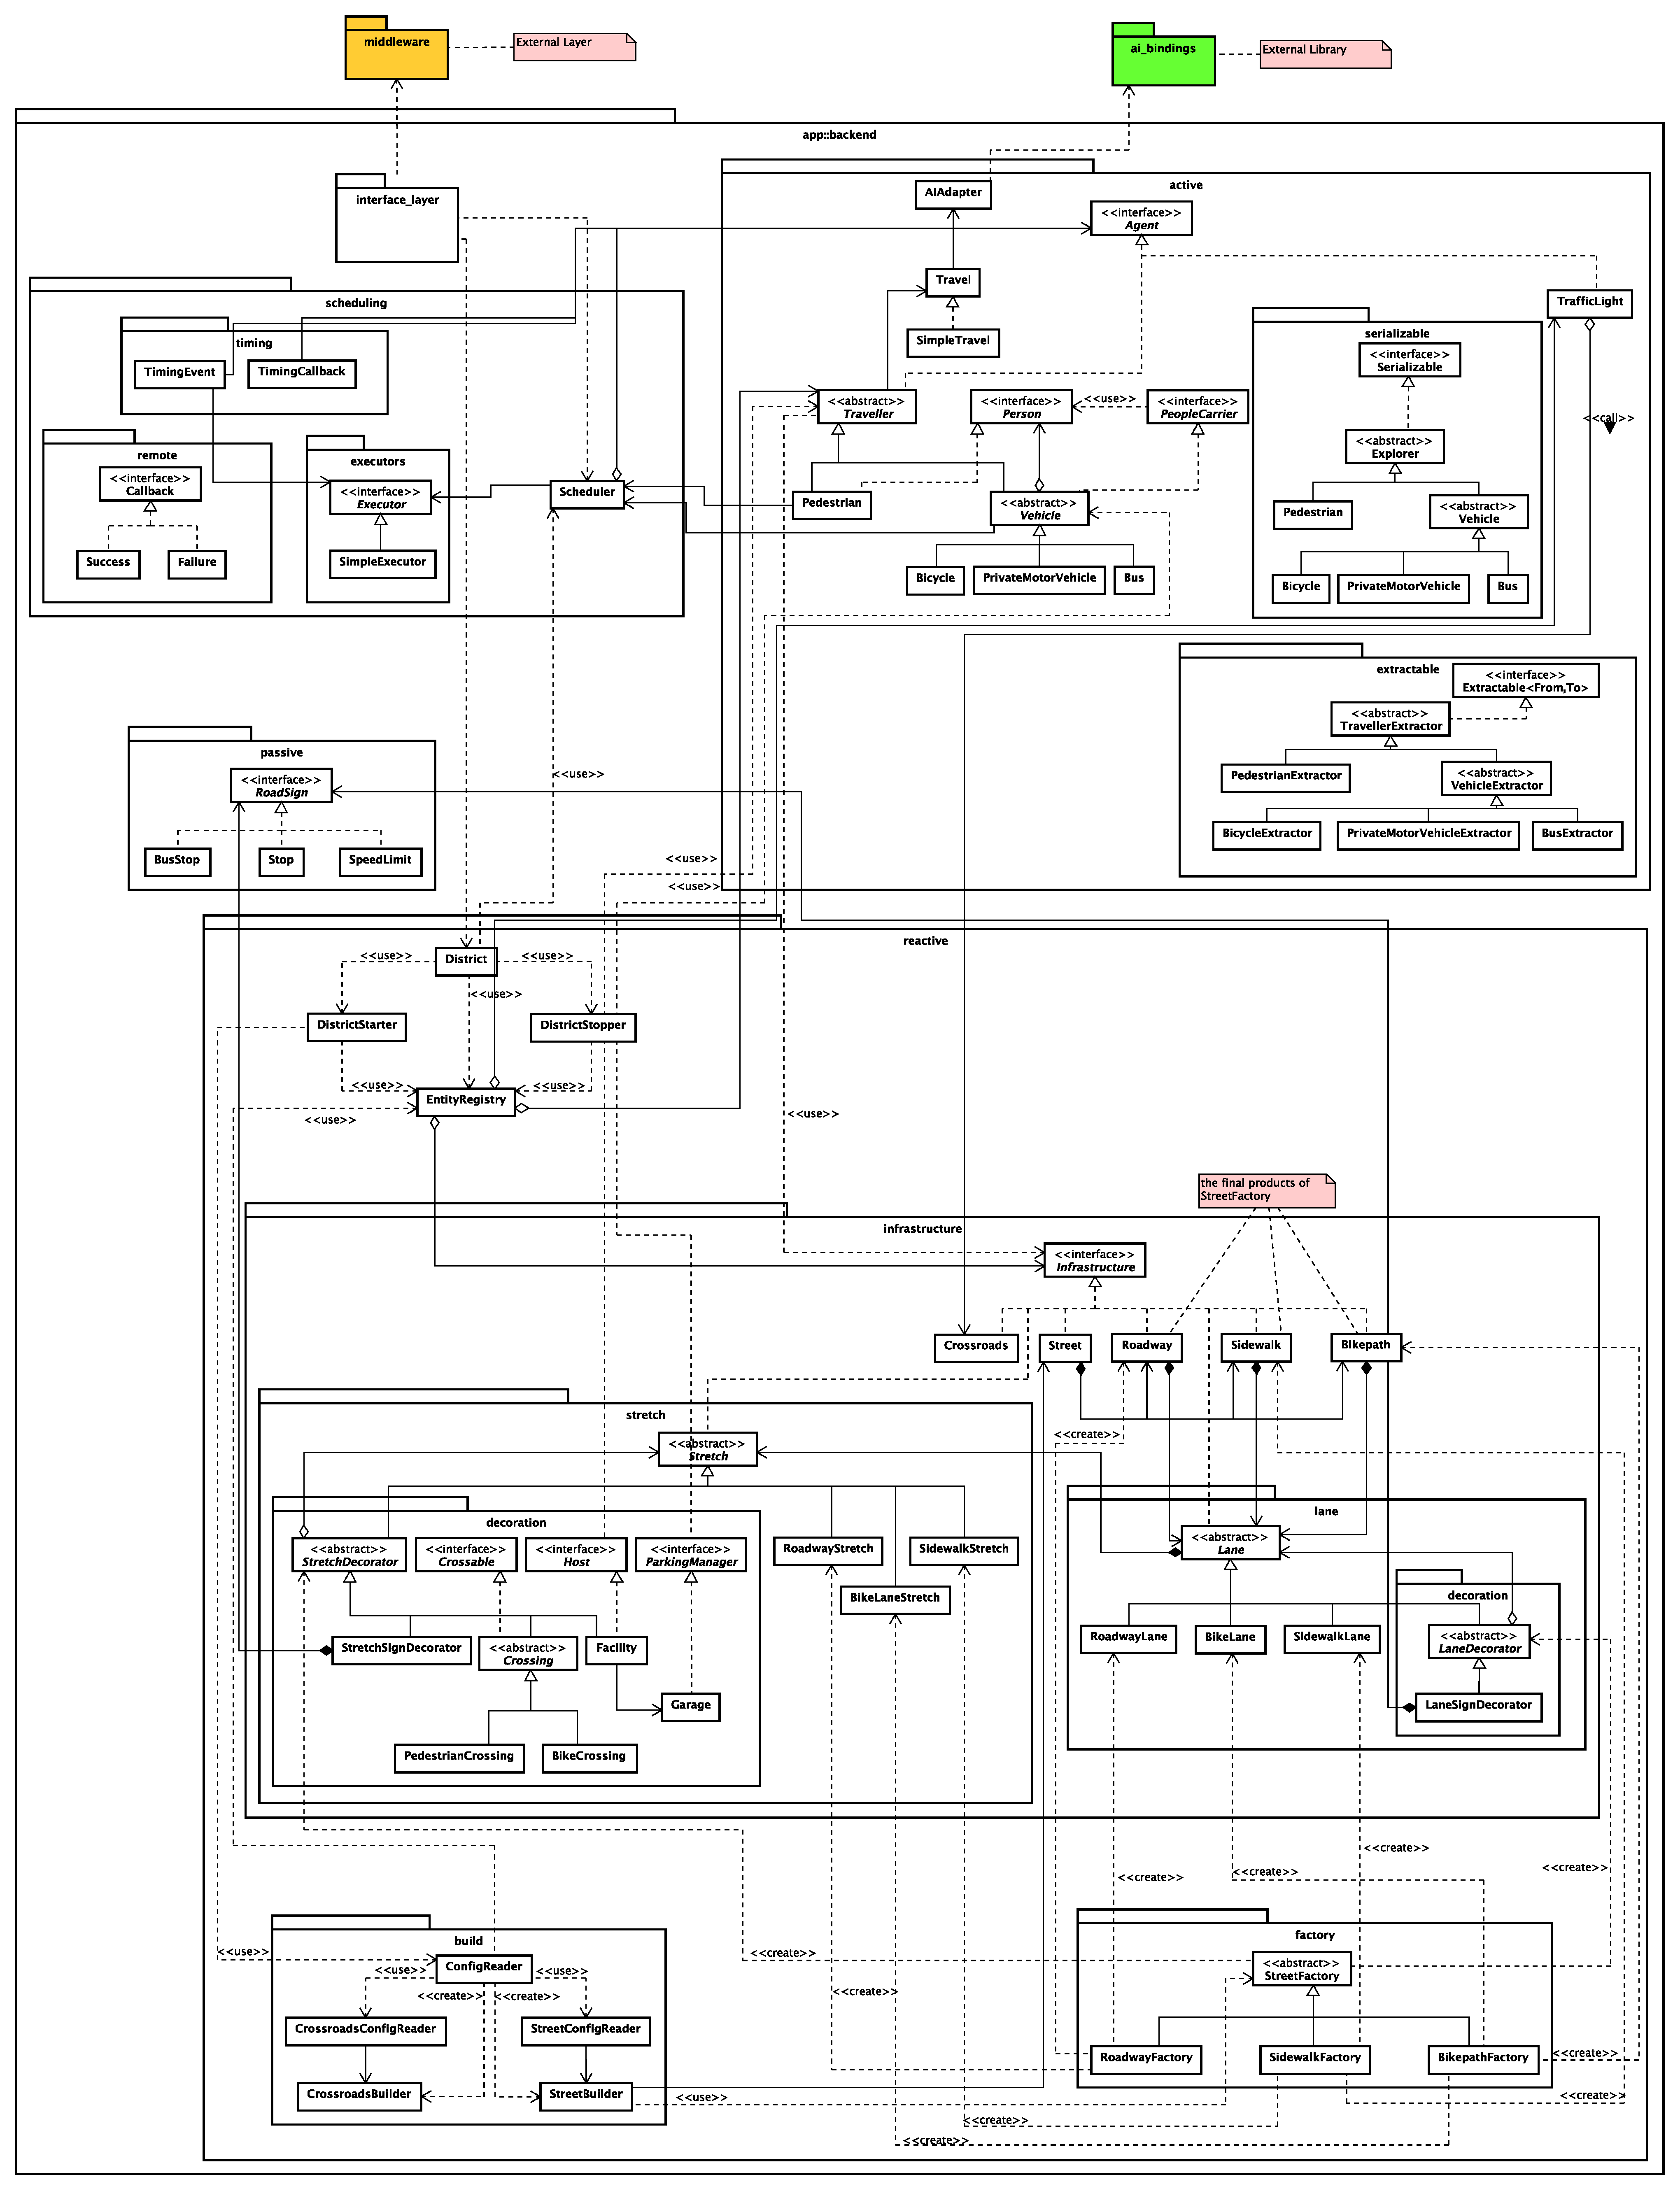
\includegraphics[width=.95\columnwidth]{images/solution/app/backend/app_backend_architecture.eps}
  \caption{Application Layer: top level design}
  \label{fig:sd-app-backend-architecture}
\end{figure}

\subsubsubsection{Active entities}
This package includes the hierarchies for active entities, along with some
additional scaffolding to make them work
(e.g., \texttt{Builders} or \texttt{Utils} packages).

At the root of this hierarchy there is the \texttt{Agent} interface, which is
used by the scheduler's worker threads to run active entities. Here we can also
find other interfaces and abstract classes, like \texttt{PeopleCarrier},
\texttt{Traveller} and \texttt{Vehicle}.

The hierarchies have been designed to be easily extensible.
In particular, the \texttt{Traveller} hierarchy has a parallel hierarchy of
\textbf{Extractors}: these modules are needed to extract state information from
the travelers when they have to be marshalled.
Separating the hierarchies allows to not affect the interface
of other travelers, the drawback of this approach consist in maintaining
two separated hierarchies.

% We used several architectural design patterns, for instance the
% \textit{Decorator} or the \textit{Strategy} patterns. For example, a private
% motor vehicle (e.g., a car) could land some of its passengers before invoking
% the traveler's superclass implementation, which makes it advance its travel.

More details about Active packages can be found in the source code itself,
which has been thoroughly commented.

\subsubsubsection{Reactive entities}
This is one of the largest packages of our system.
It contains:
\begin{itemize}
	\item all the reactive entities (streets, lanes, stretches, etc.);
	\item the builders and factories of the reactive entities;
	\item the district class, which acts as a Facade for
the whole application (except for scheduling);
	\item the entity registries and directories (subdivided by entity types);
	\item some scaffolding packages like Utils.
\end{itemize}

The important interfaces of the package are \texttt{Infrastructure} and
\texttt{Treadable}. The former represents an infrastructural object while the
latter represents a piece of infrastructure on which an agent can travel
(i.e. stretches and intersections).
In our system we consider the streets and lanes just as containers
implemented using the \textit{Composite} pattern:
\begin{itemize}
	\item a \texttt{Street} is a composition of \texttt{Way}s;
	\item a \texttt{Way} is a composition of \texttt{Lane}s;
	\item a  \texttt{Lane} is a composition of \texttt{Stretch}es.
\end{itemize}

Thus, we consider the stretch as the basic unit
of the street where an agent can travel.
Handling the concurrency at this level potentially enables
an high level of  parallelism in our system.

The other basic infrastructural entity on which an agent can travel is
\texttt{Intersection}. Each \texttt{Intersection} reserves one of its
entries for a traveler if it is a vehicle, otherwise it is just bypassed by
pedestrians and bicycles.

A \texttt{Treadable} object do not make worker threads block in its
critical regions.
Any time a traveler moves on them, a \texttt{Treadable} object attempt
to make it enter. If this
operation is successful, the traveler advances in the next piece of
infrastructure
and leaves the former one. Otherwise, the traveler is rescheduled
for a time span ahead
to retry the operation. In the latter case, the traveler does not leave
the reactive entity where he is currently in.

In this package we also implemented the decorators for stretches and lanes: they
override basic operations by composition and enrich some of them with custom
behavior. For example:

\begin{itemize}
  \item before entering a new lane it may be applied a given speed limit;
  \item before treading a stretch, further checks may be required if it is a
    part of a pedestrian/bicycle crossing.
 \end{itemize}

\subsubsubsection{Passive entities}
This package basically contains bus stops and speed limits.
Clearly, it may be extended to include other street signs, but road signs like
the one-way street signs are unnecessary due to the structure of the streets.

\subsubsubsection{Scheduling}
The scheduling package contains a pool of worker threads
which consume work items. In our
simulations, each action of an agent corresponds to a work item.

The scheduling system instantiates two executors, one for the travelers and
one for traffic lights.

These two executors are different instances of the same class.
The traffic light executor has a less number of worker threads
than the travelers executor.

We will present our scheduling component by first describing how our system
starts, then how it executes work items and how it stops.
Finally, we will have a quick look at the \texttt{Callback} hierarchy.

\paragraph{Start}

Scheduling is started asynchronously by providing a list of work items
(or \textit{agenda}), which correspond to either travelers' or traffic
lights' actions.
Scheduling will just process this list by registering events at the time
reported in the agenda.

\paragraph{Execution}

In Figure \ref{fig:schedule-execution} we show how a request to schedule
an entity is handled:

\begin{enumerate}
  \item The \texttt{Scheduler} delegates the execution of an action to
    an \texttt{Executor}: the latter is an interface which is implemented by
    the \texttt{SimpleExecutor} concrete class in our system;
  \item \texttt{SimpleExecutor} use the \texttt{Timing} package passing
  the time to defer the action as a parameter. This package
  wraps the executors inside an handler and registers the deferred callback
  in the Ada runtime using the \texttt{Ada.Real\_Time.Timing\_Events} package
  \cite{taft2006ada};
  \item When the timer expires, the Ada scheduler runs the registered handler
  which triggers the \texttt{Executor} reference to
  execute an action (the one originally delegated by the \texttt{Scheduler});
  \item If it is not stopped, \texttt{SimpleExecutor} add this action to the
    \texttt{WorkQueue};
  \item An idle \texttt{WorkerThread}, which was waiting for an item to
    execute, can dequeue the new item from the FIFO \texttt{WorkQueue}
    and consume it.
\end{enumerate}

\begin{figure}[H]
\centering
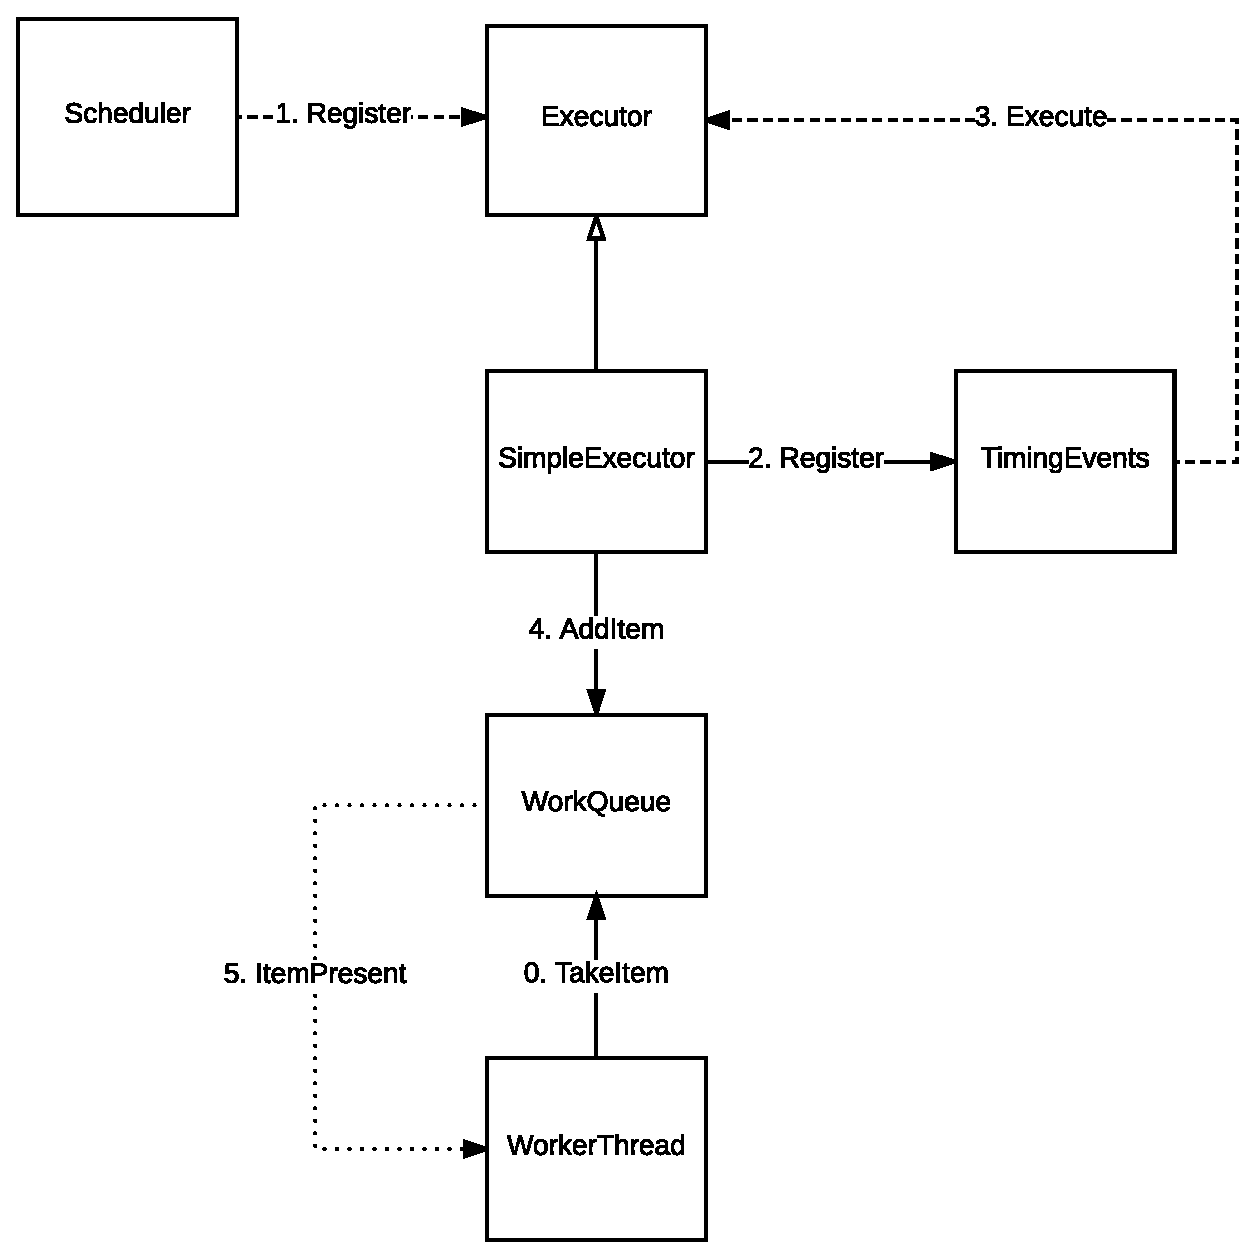
\includegraphics[scale=0.5,keepaspectratio]{images/solution/app/backend/scheduling-execution.eps}
\caption{Execution of a work item}
\label{fig:schedule-execution}
\end{figure}

\paragraph{Termination}

In Figure \ref{fig:schedule-termination} we show how a request to schedule
the termination of an entity is handled:

\begin{enumerate}
  \item The \texttt{Scheduler} asks the \texttt{Executor}s to shutdown;
  \item \texttt{SimpleExecutor} stops itself and then loads in the work queue
    one poison pill for each worker thread of its thread pool;
  \item Eventually, each worker thread will fetch a poison pill from the work
    queue;
  \item When trying to consume a poison pill, a worker thread will stop
    itself on a barrier between it and the Executor;
  \item Finally, when all the workers are stopped, the Executor is unblocked
    from the the barrier.
\end{enumerate}

\begin{figure}[H]
\centering
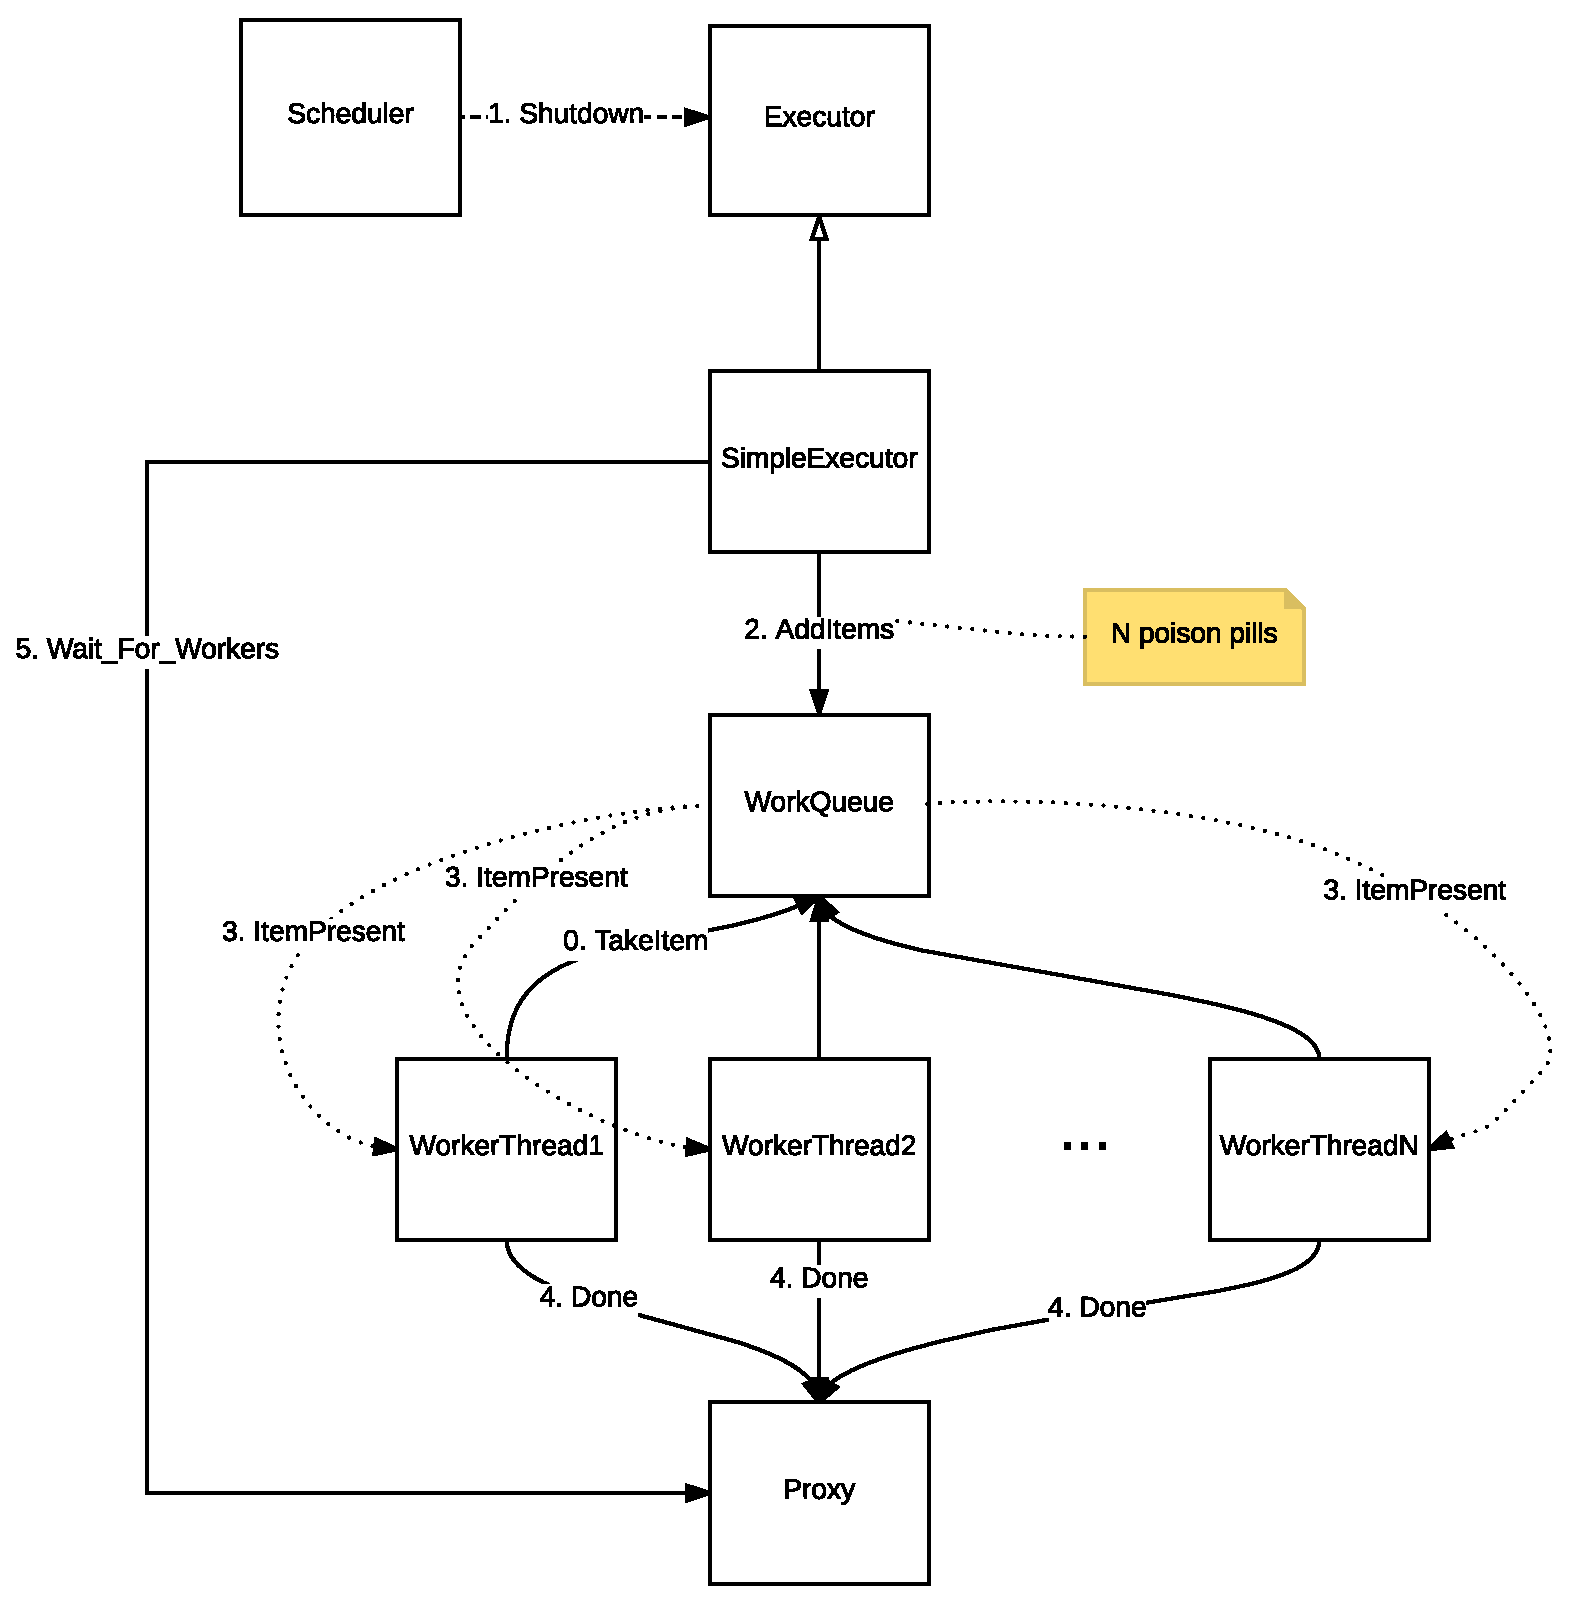
\includegraphics[scale=0.5,keepaspectratio]{images/solution/app/backend/scheduling-termination.eps}
\caption{Scheduling termination}
\label{fig:schedule-termination}
\end{figure}

\paragraph{Callbacks}

As we can see from the code, we implemented four callbacks (actually, two
pairs of success/failure callbacks).
We introduced this mechanism in our system to avoid
communication deadlocks on synchronous remote calls.
Indeed, during some simulation it may happen
that all the worker threads are
blocked on several remote calls which receives no response.
In this case the scheduling system would block and all the agents would not
been scheduled.

Each callback is inserted in a pending requests map
and referenced by the message identifier.
IL is in charge of handling the callbacks inserted in the map based on the
received replies.

\subsubsection{Interface Layer}

Figure \ref{fig:impl-il-arch} provides an high level view of
the Interface Layer (IL) components.

\begin{figure}[H]
  \centering
  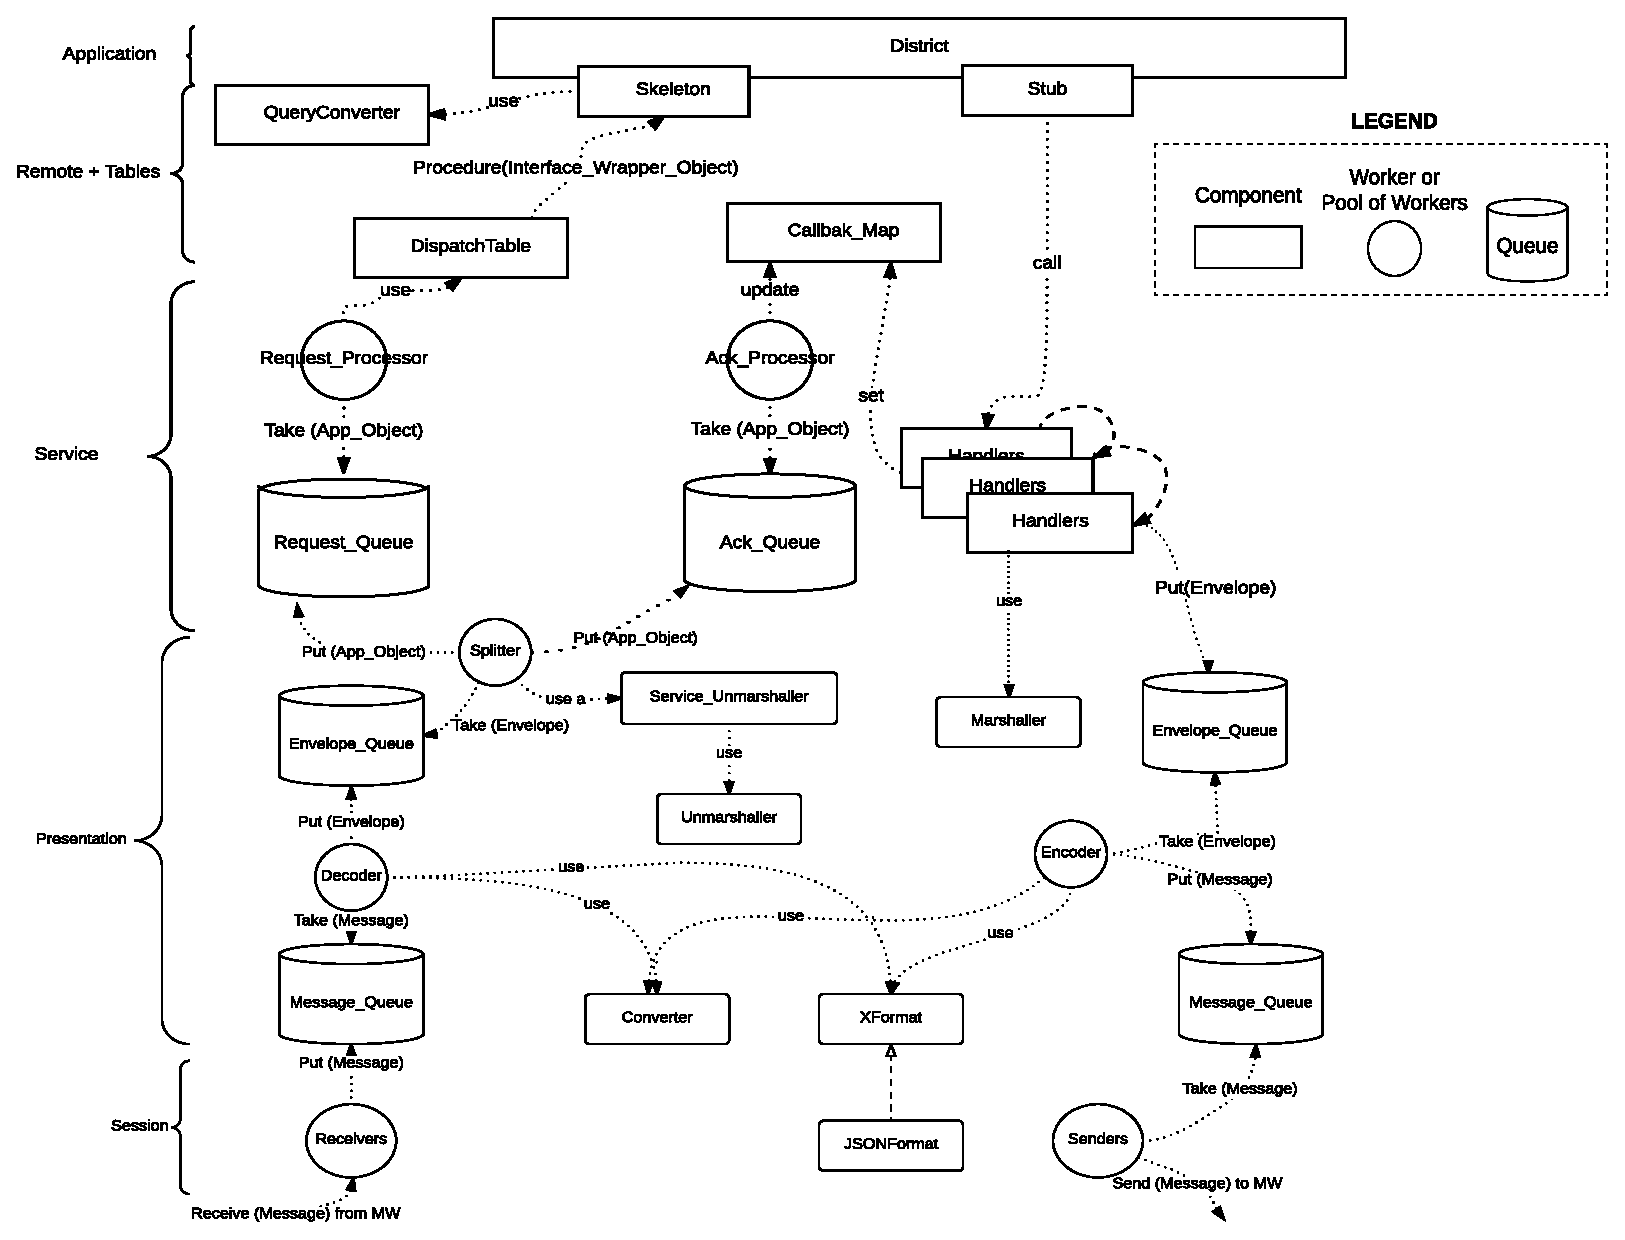
\includegraphics[width=\columnwidth]{images/solution/il.eps}
  \caption{Interface Layer architecture}
  \label{fig:impl-il-arch}
\end{figure}

IL enables the Application Layer to communicate with other applications
transparently without knowing if they are local or remote. We encapsulate the
application data as message payload while
different sublayers of IL manipulate different fields of the
message header.
This layered approach has been inspired by the TCP/IP and ISO/OSI models, in
which the layers communicate in two directions:
\begin{itemize}
	\item \textbf{horizontally:} manipulating the same fields of the header;
	\item \textbf{vertically:}  - passing the packet to the next
layer, which is charged with different responsibilities.
\end{itemize}
Also, IL is completely asynchronous because each of its sublayers has its own
thread pool. Furthermore, each thread pool is controlled by a master thread which
runs in an event loop consuming messages from its own incoming
queue. For example, the receiver can handle potentially multiple concurrent
requests by delegating each one of them to its worker threads.
After a worker has
completed the assigned task it is pushed back on the receiver's local stack,
ready to be reused.


In the following we list the sublayers which compose IL in
bottom up order:

\begin{itemize}
  \item \textbf{Session Layer:}
  handles remote connections through TCP sockets;
  \item \textbf{Presentation Layer:}
  handles messages formatting and conversions;
  \item \textbf{Service Layer:}
  converts remote requests into procedure calls
  by leveraging a skeleton object.
  Also, it offers the specular service through a stub object plus a pipeline
  of handlers. For each request, the former compose a specific pipeline
  of handlers transparently to the Application Layer.
  The handlers are used to incrementally construct the message by adding
  header fields, wrapping the data into a payload field and finally putting
  the message in the first queue which goes downwards (towards the middleware).
  \item \textbf{Remote Layer + Tables:}
  It contains the tables used
  to dispatch the remote calls and the callback map of pending requests.
  A pending request is a synchronous requests which may trigger one of
  the following behaviors:
  \begin{itemize}
  	\item retransmission on timeout;
  	\item a local retry on failure - retry on the local district with
  	the next action which could be a repetition of the last executed action;
  	\item a local clean up on success - remove the retained data from the local
  	district. The message has been successfully sent.
  \end{itemize}
  With pending request we are not reinventing a weakened version
  of TCP retransmission timers as it might seem.
  Indeed, we have concretely faced network connection errors during
  the communication
  with the middleware layer. This was caused by occasional failures or network
  problems subsequently fixed by the system itself
  (i.e., the docker swarm node).
  However,
  we preferred to give the responsibility of these synchronous messages to IL
  for two reasons:
  \begin{itemize}
  	\item it is the layer which has the highest probability of not losing them.
  	Indeed, the communication with the Application Layer happens through
  	local procedure
  	calls. Also, the TCP communication with the middleware layer could lead to
  	lose messages;
  	\item the data wrapped in the messages are important for the
  	application which can not afford to lose them. Indeed, a lost message
    could mean a missing pedestrian in the system. Thus, a failure
  	or a timeout has to trigger a reaction as soon as possible because
  	the latency introduced in the communication can lead to a significant
  	time drift for the end user (e.g., a set of travelers blocked with
  	apparently no reason). This could undermine the principle of viewing the
  	whole distributed system as one single unit.
  \end{itemize}
\end{itemize}
\subsubsection{Bootstrap}

The bootstrap process consists of two ordered and separated processes:

\begin{enumerate}
  \item \textbf{Initialization:} instantiates and configures the necessary
    resources for the application;
  \item \textbf{Activation:} starts the application.
\end{enumerate}

Clearly, the activation phase depends on initialization.
While the initialization process is automatically triggered at node creation,
this is not the case for activation, which is instead triggered by the
middleware.
Moreover, at the Application Layer level, we have to consider the dependencies
among the entity types (which are depicted in Figure
\ref{fig:sd-entity-types-deps}).

The overall bootstrap process, which mimics UNIX init \cite{online-tlsag},
is divided in two ordered parts:
\begin{enumerate}
  \item \textbf{Init:} initialize all the sublayers of each macro layer,
  following a bottom up approach (from \verb|interface_layer.session| to
  \verb|application.scheduling|).
  The initialization order is given by the fact that the upper
  layers need the services provided by the underlying layers to work
  correctly (Figure \ref{fig:sd-app-init});
  \item \textbf{Start:} IL forwards the start message sent from the
  middleware to the Application Layer.
  Therefore, this event is exclusively triggered by the middleware.
\end{enumerate}

\begin{figure}[H]
  \centering
  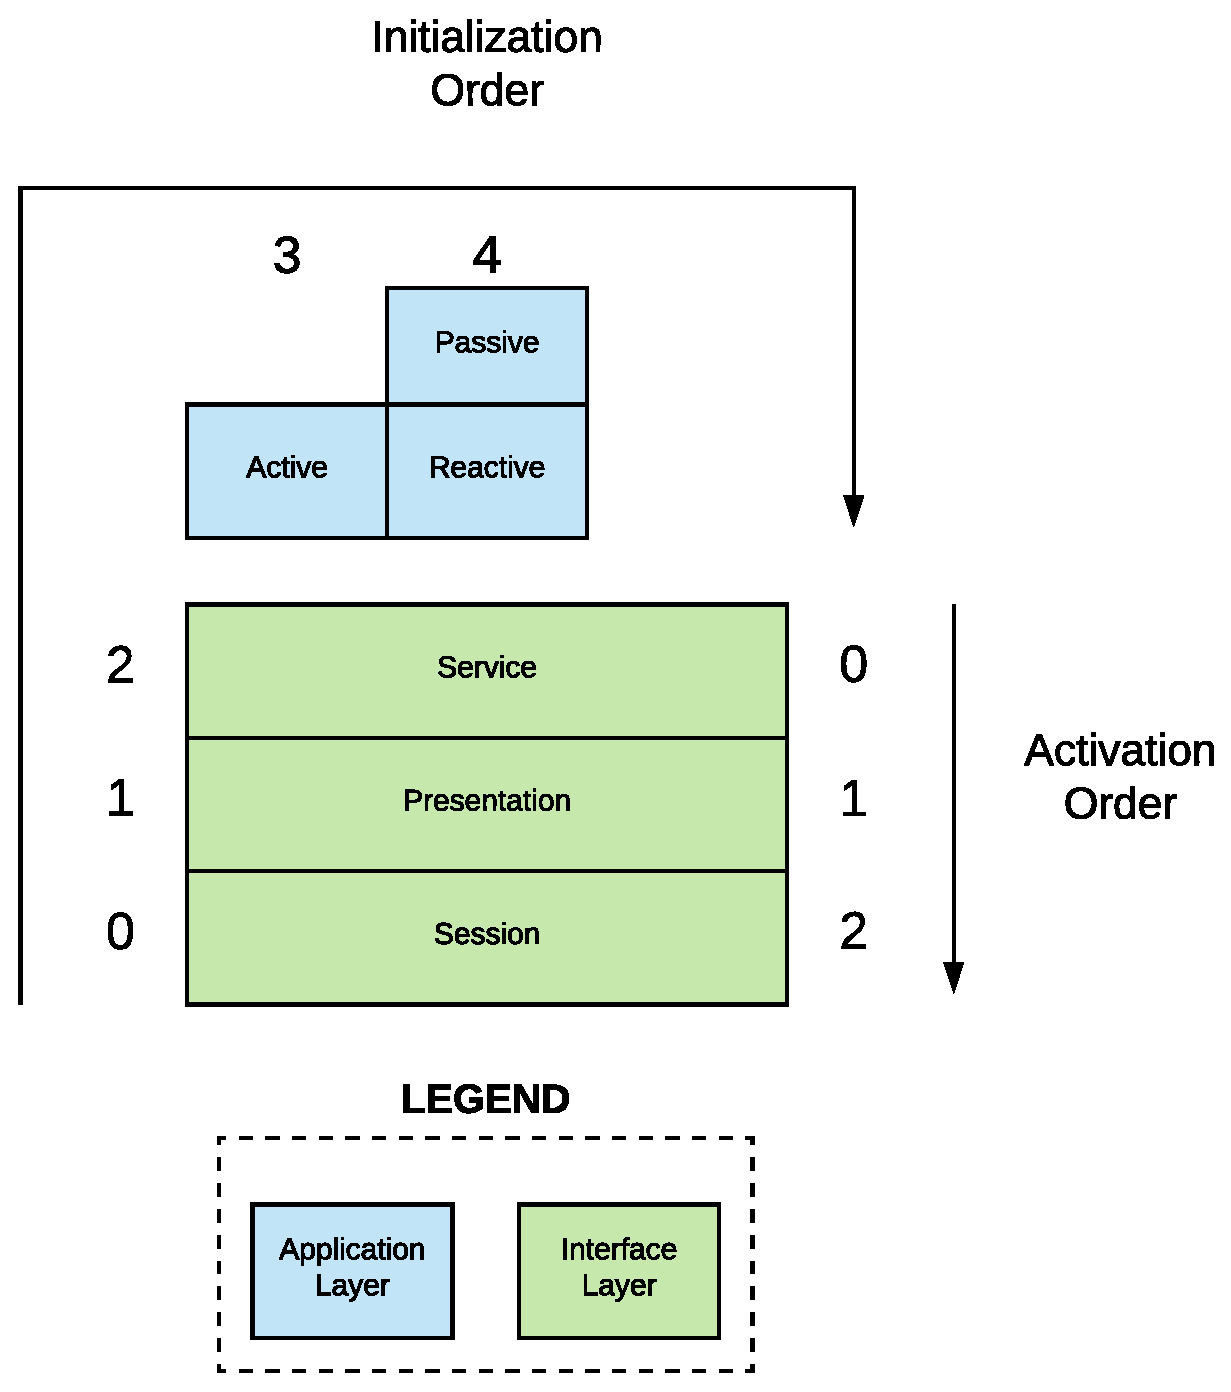
\includegraphics[scale=0.5,keepaspectratio]
    {images/solution/init_activate.eps}
  \caption{Application Bootstrap - Init}
  \label{fig:sd-app-init}
\end{figure}


\subsubsubsection{Init}

Each application node contains the \textit{Init} process,
which is the parent of all the application processes.
The execution steps of \textit{Init} are depicted in Figure
\ref{fig:sd-app-init}.
It instantiates the resources of each layer, thus making
Interface Layer and Application Layer transit from the \verb|inactive|
to the \verb|ready| state.
For example, each sublayer of Interface Layer instantiates its own pool of
LWPs\footnote{lightweight processes}.

The Application Layer initialization completes in the following order:

\begin{enumerate}
  \item \textbf{Active:} the entities which move in the city (e.g.,
    pedestrians);
  \item \textbf{Reactive:} the infrastructure of the city (e.g., streets);
\end{enumerate}

The Scheduling package, which manages the execution order for the events of the
Application Layer, does not require an initialization step. This package
will be started directly through the start message.


Since the \textit{Passive} entities are stateless and
logically belong to \textit{reactive} entities (e.g., speed limits belong to
roads), they will be instantiated along with them
(Figure \ref{fig:sd-entity-types-deps}).

When \textit{Reactive} completes its initialization, \textit{Init}
signals the Application layer completion to each sublayer of Interface Layer
in the following order:

\begin{enumerate}
  \item \textbf{Service:} provides activators and pipelines services to
    application layer;
  \item \textbf{Presentation:} provides data conversion services;
  \item \textbf{Session:} provides network connection services (e.g., senders
  and receivers).
\end{enumerate}

\textit{Init} triggers the transition of each IL sublayer state from
\verb|ready| to \verb|active|.
The activation order is extremely important to proactively avoid
message losses between remote nodes.
Indeed, at this stage, the application layer is
not able to generate or receive messages because the start message has not
been sent by the middleware. Obviously, IL is a reactive component
of the backend subystem. Thus, its \verb|active| state means
that all the workers of IL have started their event loop.
Their loop execution is triggered each time a
message arrives. Indeed, the workers are blocked on unbounded synchronized
queues which have been designed to be thread safe \cite{taft2006ada}.


The service and the presentation layer are activated before the session layer;
the latter exposes a remote communication channel through TCP
sockets.
Finally, the application is ready to communicate because both of its layers
has been activated.

Now, the Application waits the \verb|start|
message from the middleware.


A crash of the \textit{Init} process, occurring before the end of the
bootstrap, is detected by the middleware layer. The expiration
of a timeout triggers a retransmission from the middleware side.
Note that this model should also work for a bootstrap which is executed
starting
from a valid snapshot of the system, with the only difference consisting in
divergent values of the configuration file.
Indeed, for each simulation we will use a set
of configurations which is going to be different for each city.

\subsubsubsection{Start}

When \textit{Init} completes, the Application Layer is in a \verb|ready| state
while Interface Layer is in an \verb|active| state.
The first message sent by the middleware towards the Interface Layer is a
\verb|start| message which triggers the Application Layer activation.

The \verb|start| message kickoffs the scheduler, causing it to load the set
of actions declared in its configuration file. An action is a $<$\verb|agent|,
\verb|time_span|$>$ pair, i.e., the active entity \verb|agent| will act in
\verb|time_span| milliseconds.

\subsubsubsection{Termination}
When describing the shutdown of the whole system, we assumed 
the application terminates gracefully.
In this section we show the algorithm that is used to achieve this goal.

As we can see from figure \ref{fig:app-proc-tree}, the termination follows the
opposite order of the bootstrap.

\begin{enumerate}
  \item The \textit{Master} task $M$ stops active entities, e.g. pedestrians;
  \item After stopping active entities, $M$ saves their state into a file;
  \item $M$ saves into a file the state of reactive entities. 
  It is important to notice their internal state is now safetely savable, 
  since no active entities can modify it anymore;
  \item $M$ sends an \texttt{app\_shut} message to the middleware;
  \item $M$ terminates itself and the entire application consequently stops.
\end{enumerate}

The middleware layer can request the application to stop via the
\texttt{app.shutdown} call.

The last operation the \textit{Master} task does is to send a message for apprising
the middleware layer of the successful termination of the application one.
Similarly to the bootstrap phase, the middleware expects to receive this
message within a certain amount of time. 
In order to do so, when sending the message, $M$ also starts a timeout.
Wherefore if it expires before receiving a response message from the middleware layer, 
it calls again the \texttt{app.shutdown} procedure the application exposes.

\subsubsubsection{Interaction between entities}

The application contains several interactions among entities that have to be
specified in order to understand well how to approach different problems.

\paragraph{Entering a road} Moving entities enter a road by entering a stretch
that is located at the beginning of the road and that is treadable by their
specific entity type.

\paragraph{Entering a road stretch} Moving entities who want to enter a new
road stretch can do it whenever there is room for them in that stretch. In
particular, a roadway stretch can be trod for at most one vehicle at the same
time.

\paragraph{Zebra crossings} Vehicles which want to enter a road stretch that
has zebra crossings painted on it has to wait for pedestrians or bikes to free
all stretches of that particular crossing.

\paragraph{Changing roadway lane} A vehicle that is on the i-th road stretch
which wants to change lane has to check whether the (i+1)-th stretch in the
wanted direction is free.

In that case, the vehicle enters the stretch of the other lane; otherwise, if a
timeout expires before a vehicle is able to change lane, then it gives up on
it and proceeds forward to the next stretch.

\paragraph{Crossroads} Every road that is connected to a crossroads is marked
with a cardinal point (N/E/W/S). The crossroads holds all the logic necessary
for vehicles to follow the yield rules we described in
\ref{sec:pa-domain-problems}.

There could be a situation in which there is a standstill, for example when
four cars want all to go straight in a four-way crossroads. In this case, the
crossroads will make a car yield the right-of-way to another one.

Pedestrians can only walk on the corner of the crossroads, thus passing to the
adjacent piece of road (e.g. a pedestrian that is coming from the ``southern''
side of the western road can only enter the southern street on the ``western''
side).

\paragraph{Entering a building} When a moving entity is in the stretch where
there is the entrance of a building, then it may enter the building.

If the moving entity is a vehicle, it has to wait for all other entities who
are in the intermediate stretches to move away.

\paragraph{Exiting a building} When a moving entity is exiting a building, it
has to check whether there is room for her to move out.

If the entity is a vehicle, it has to yield the right-of-way to upcoming
vehicles and to wait that eventual sidewalks or bicycle path stretches in front
of the building are free too.

\paragraph{Choosing to use a vehicle} An entity $e$ who wants to leave a
building $b_e$ to a destination $d_e$ may randomly decide not to travel by
foot. She can leave only if:

\begin{itemize}
  \item the path from $b_e$ to $d_e$ does not include any destination of other
    people who are leaving from $b$ and viceversa. Otherwise, they would share
    the vehicle if there is enough room;
  \item there is an available vehicle in $b$; and
  \item the capacity of the destination building $d_e$ is greater than the sum
    of all vehicles in it and the ones which are arriving to that building.
\end{itemize}

If all these conditions are met, then:
\begin{itemize}
  \item the entity may exit the building and travel using a vehicle; and
  \item $d_e$ now ``books'' a place for the vehicle driven by $e$.
\end{itemize}

\paragraph{Waiting for a bus} A pedestrian may randomly decide to wait for a
bus if she is on a bus stop stretch.

Firstly, she checks whether the buses that stops at that stretch match (even
partially) her path. If at least one of them does, then she wait for a limited
amount of time for a bus to arrive.

If this timeout expires, then she continues travelling by foot to the next
stretch.

\paragraph{Boarding a bus} When a bus arrives at a bus stop, then a waiting
entity will board it only if:

\begin{itemize}
  \item there is enough room for her; and
  \item this bus shortens the expected route for her.
\end{itemize}

\paragraph{Getting off a bus} A person $p$ will get off a bus when it reaches
the last stop $s$ such that $s$ belongs to the route of $p$.

\paragraph{Respecting street code} Roads and crossroads will contain all the
necessary logic to make moving entities follow the street rules.

\paragraph{Performing an overtaking} This action is possible only when a
vehicle is able to change lane. It might be triggered by a timeout which
expires when it is waiting too much for entering the next straightaway stretch.

When a vehicle tries to overtake another one, it will always try to return to
the lane where it started the operation before entering the last stretch.
% look for "manovra" translation

% \paragraph{Uber} % Is it a TODO?


% Architectural overview
\subsubsection{High Level Design}

\subsubsubsection{Application Layer}

Figure \ref{fig:sd-app-backend-architecture} provides an architectural overview
of the classes which compose the application layer.
The main packages have been named according to Table \ref{tab:entity_type}.

\begin{figure}[H]
  \centering
  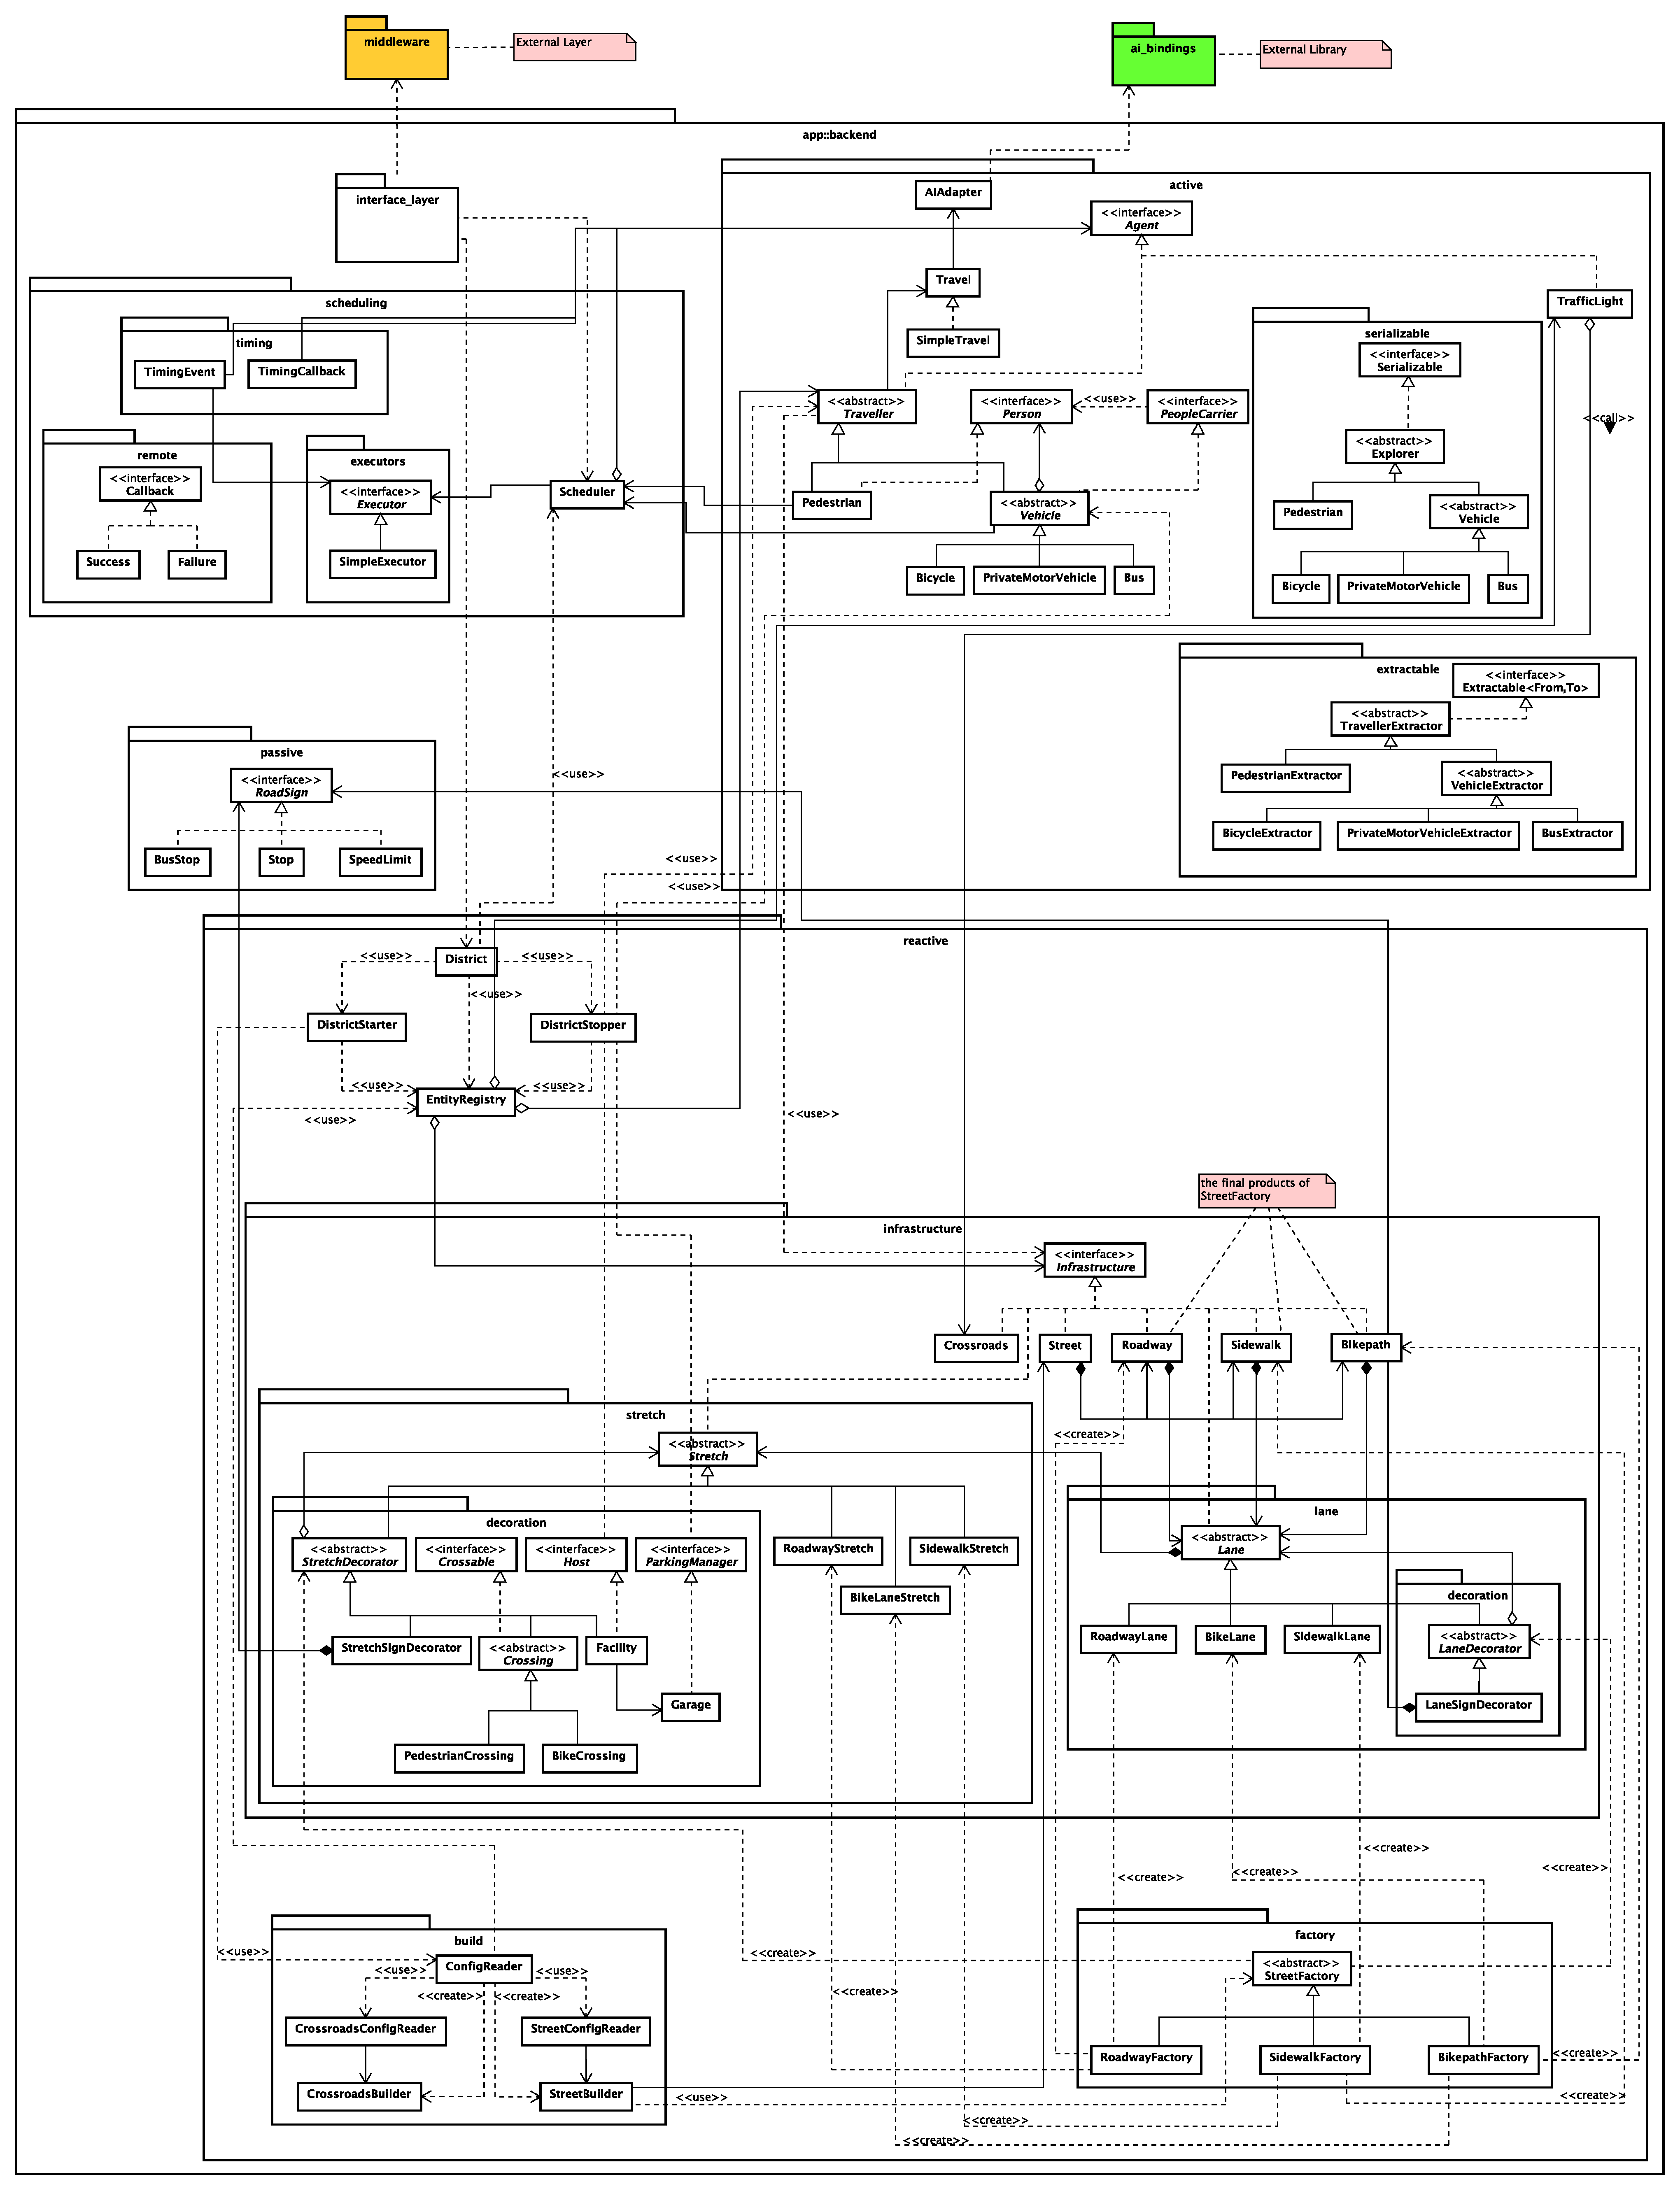
\includegraphics[width=.95\columnwidth]{images/solution/app/backend/app_backend_architecture.eps}
  \caption{Application Layer: top level design}
  \label{fig:sd-app-backend-architecture}
\end{figure}

\subsubsubsection{Interface Layer}

Figure \ref{fig:impl-il-arch} provides an high level view of
the interface layer components and their interactions.

\begin{figure}[H]
  \centering
  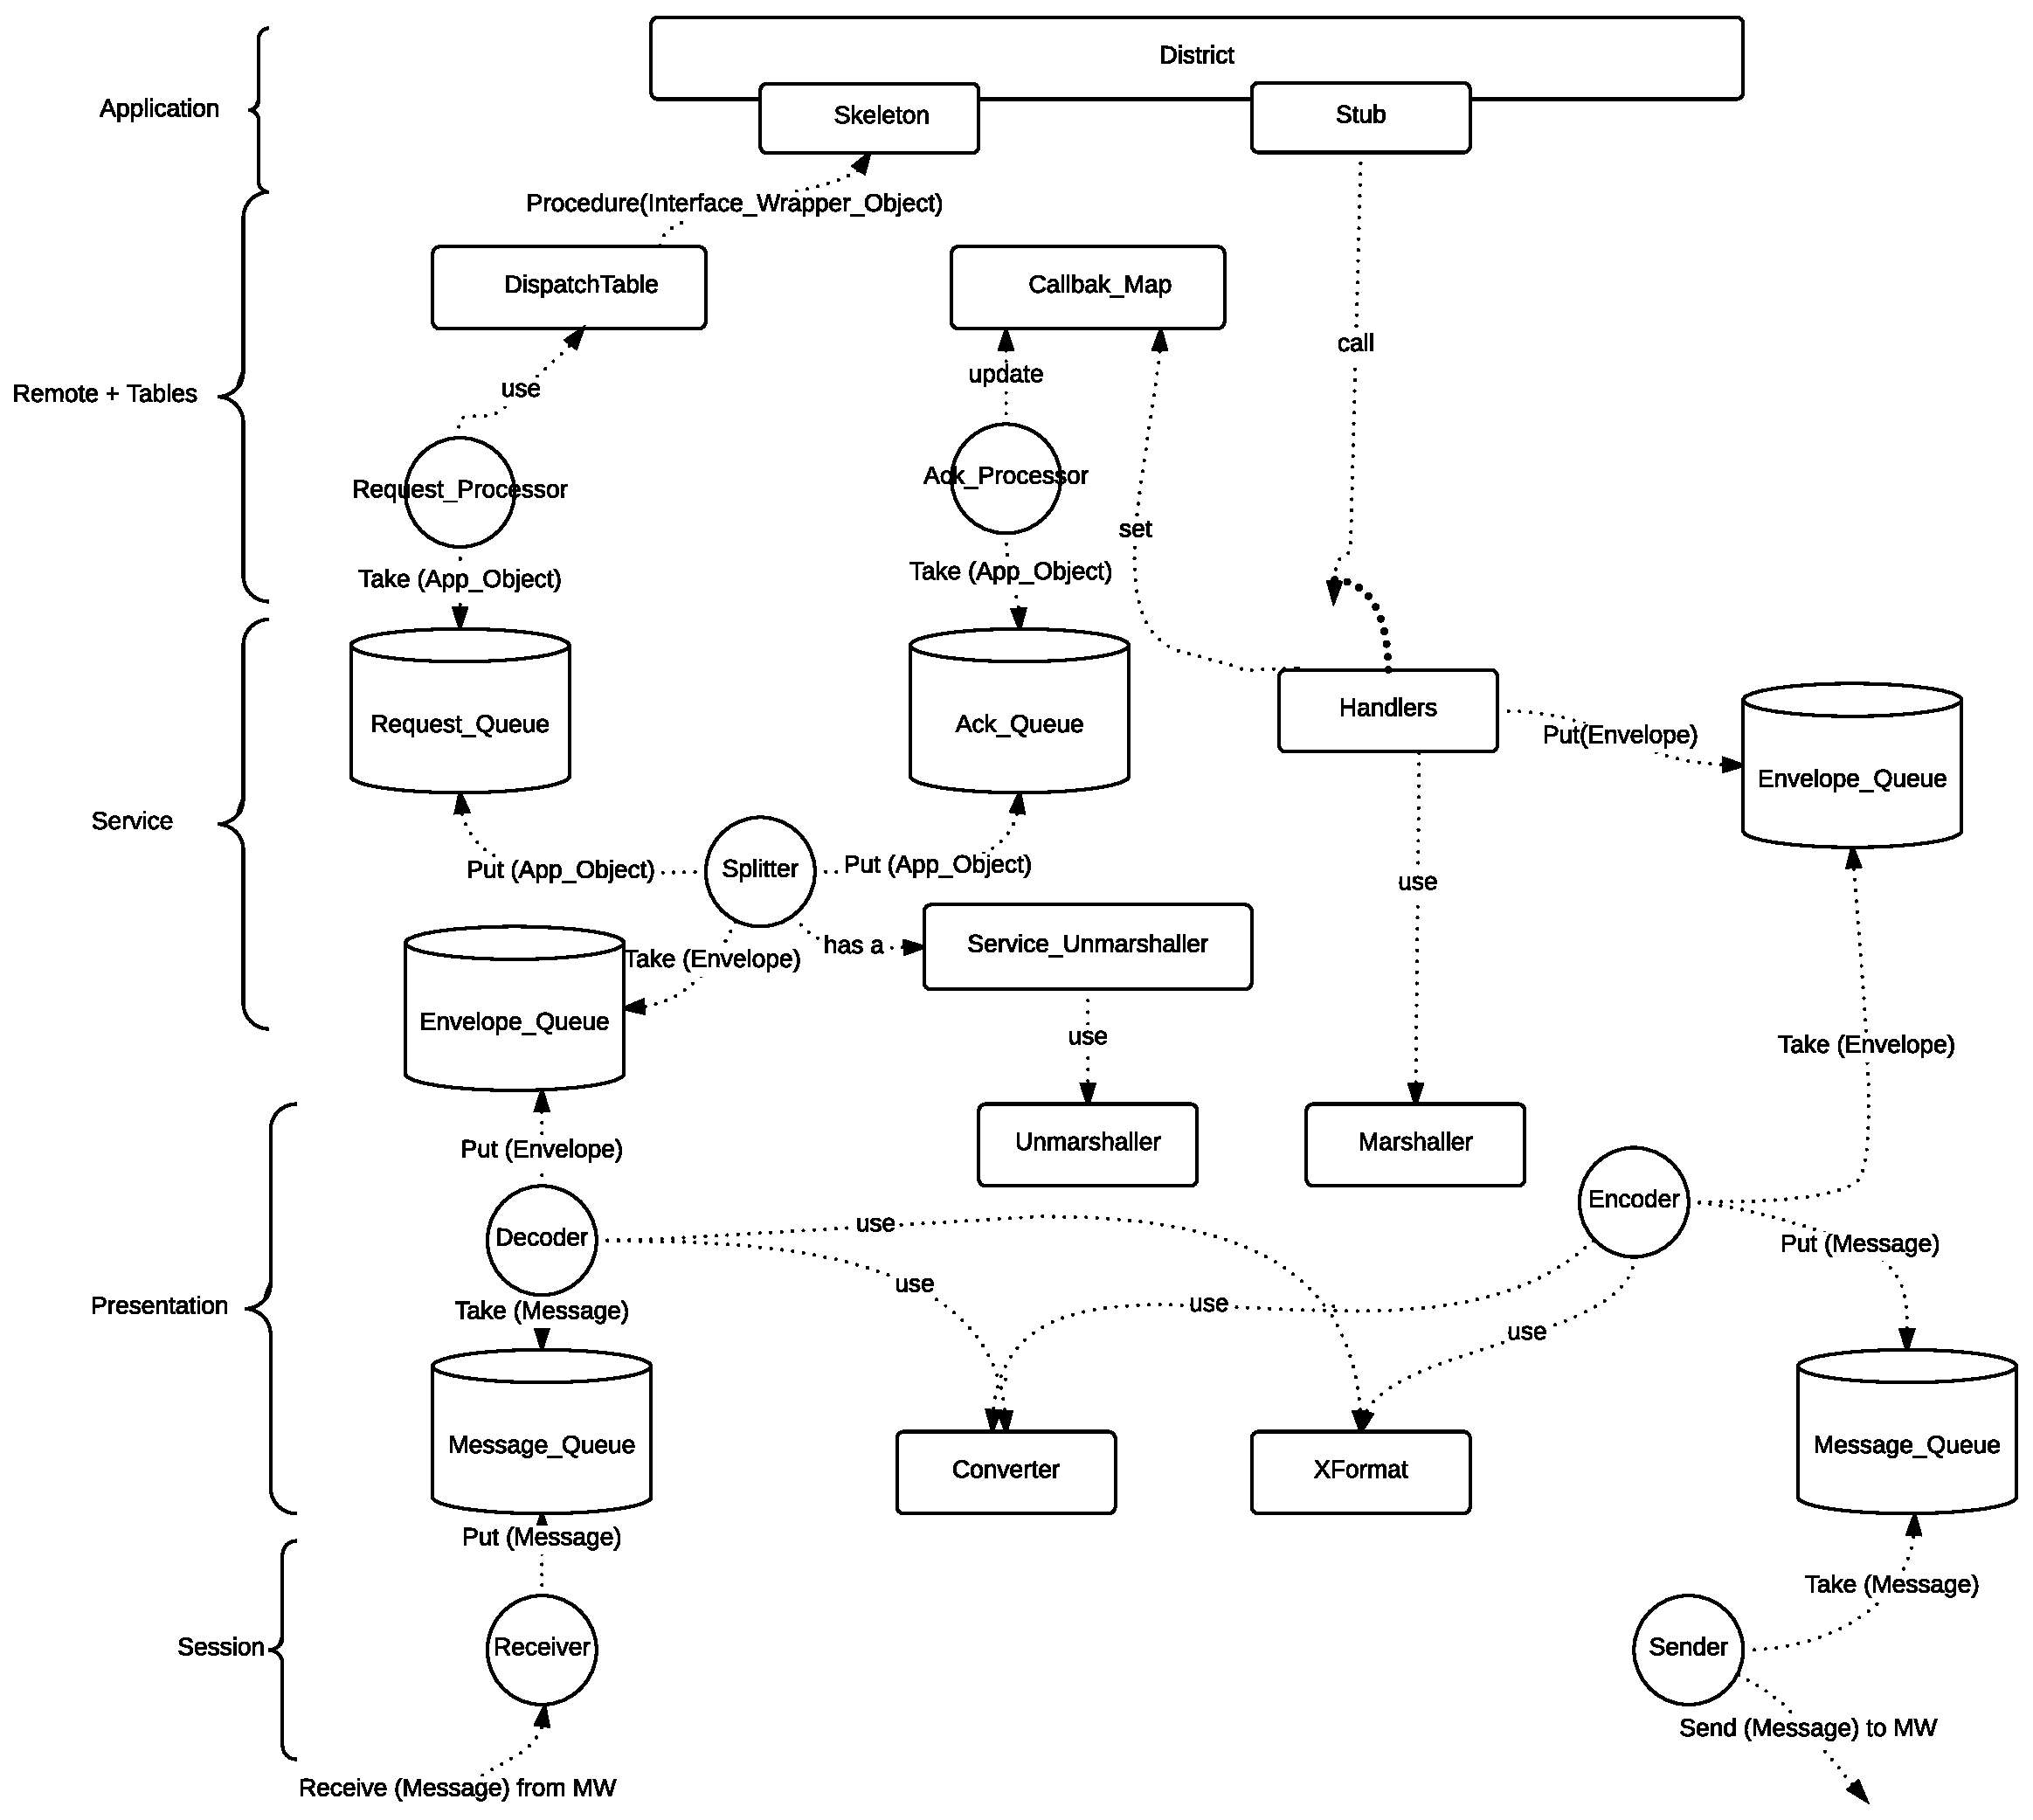
\includegraphics[width=\columnwidth]{images/implementation/il-overall.eps}
  \caption{Interface Layer architecture}
  \label{fig:impl-il-arch}
\end{figure}


% Detail design
\subsubsection{Detailed Design}

\paragraph{Types of entities}
Three types of entities have been identified
\begin{itemize}
  \item \textit{Active}: entity capable to start an action by itself if provided 
the necessary computational resources;
  \item \textit{Reactive}: entity that only reacts to provided inputs, 
not capable to start an action by itself;
  \item \textit{Passive}: a stateless entity.
\end{itemize}
\begin{table}[H]
\centering
\begin{tabular}{|l|l|}
\hline
\rowcolor{BlueGreen}
Type     & Entities                                 \\ \hline
Active   & pedestrian, car, bus, bicycle, semaphore \\ \hline
Reactive & road, crossroads, house                   \\ \hline
Passive  & road signs                               \\ \hline
\end{tabular}
\caption{Types of entities}
\label{tab:entity_type}
\end{table}
The entities have the following dependencies:
\begin{itemize}
  \item \textit{Active} provides inputs to \textit{Reactive} (solid line);
  \item \textit{Active} and \textit{Reactive} can use \textit{Passive}, the dependency is not strict (dashed line).
\end{itemize}
\begin{figure}[H]
  \centering
  \includegraphics[width=.35\columnwidth]{sections/images/solution/entity_type_dependency.eps}
  \caption{Dependencies between entity types}
  \label{fig:sd-entity-types-deps}
\end{figure}

\subsubsection{Detailed Design}
\subsubsubsection{Interface}
\subsubsubsubsection{Application}
\begin{figure}[h]
\centering
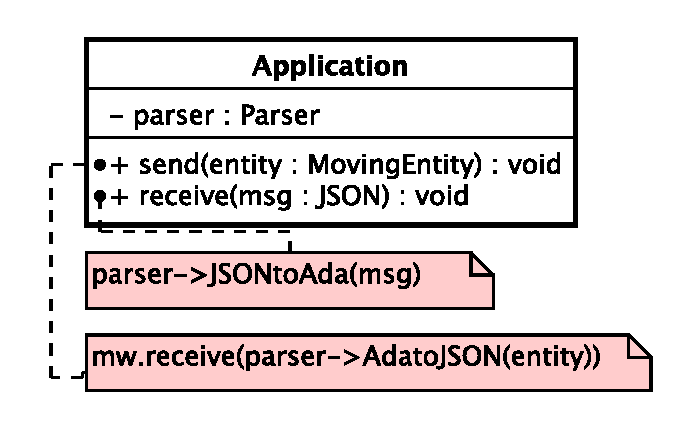
\includegraphics[scale=0.6,keepaspectratio]{images/solution/application.eps}
\caption{App::Interface::Application}
\label{fig:sd-app-application}
\end{figure}
\FloatBarrier
\begin{itemize}
  \item \textbf{Description} \\
    It represents a lightweight interface to communicate with the middleware layer.
  \item \textbf{Attribute}
  \begin{itemize}
    \item \texttt{- parser: Parser} \\
The parser object used to convert JSON data to Ada instructions and vice versa.
  \end{itemize}
  \item \textbf{Operation}
  \begin{itemize} 
    \item \texttt{+ send(entity: MovingEntity)} \\
Sends messages to the middleware layer. Before sending the message to the
middleware it converts the entity into a JSON message using the parser.
    \item \texttt{+ receive(msg: JSON)} \\
Receives a JSON messae from the middleware layer. It invokes the parser 
passing the message as parameter.
  \end{itemize}
\end{itemize}

\subsubsubsubsection{Parser}
\begin{figure}[h]
\centering
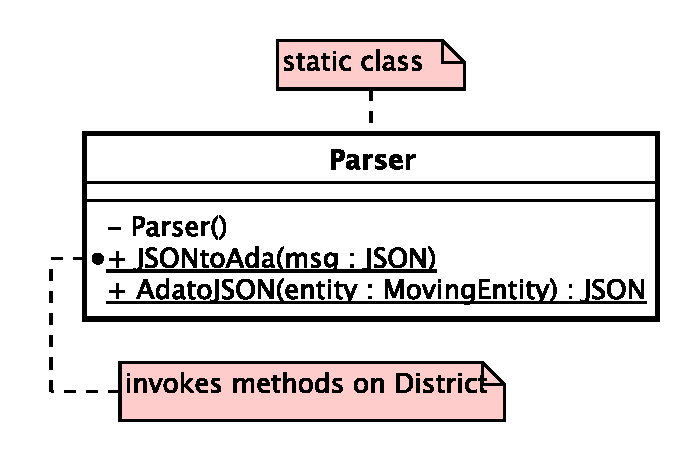
\includegraphics[scale=0.6,keepaspectratio]{images/solution/parser.eps}
\caption{App::Active::Parser}
\label{fig:sd-app-parser}
\end{figure}
\FloatBarrier
\begin{itemize}
  \item \textbf{Description} \\
    It represents a parser which converts JSON messages to Ada statements and vice versa.
  \item \textbf{Attribute}
  \begin{itemize}
    \item \texttt{- district: District} \\
The district object used as facade for the application layer.
  \end{itemize}
  \item \textbf{Operation}
  \begin{itemize} 
    \item \texttt{+ JSONtoAda(msg: JSON)} \\
Converts the JSON message to Ada statements invoking district.
    \item \texttt{+ AdatoJSON(entity: MovingEntity) : JSON} \\
Converts a moving entity into a JSON message returning the message as result.
  \end{itemize}
\end{itemize}

\subsubsubsection{Active Entity}
\subsubsubsubsection{Moving entity}
\begin{figure}[h]
\centering
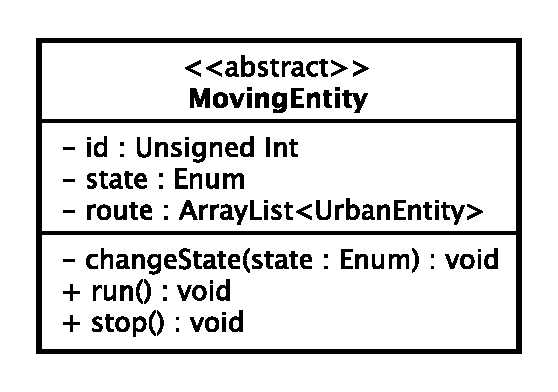
\includegraphics[scale=0.6,keepaspectratio]{images/solution/moving_entity.eps}
\caption{App::Active::MovingEntity}
\label{fig:sd-app-movingentity}
\end{figure}
\FloatBarrier
\begin{itemize}
  \item \textbf{Description} \\
    It represents an entity that moves through the city, consuming its 
route at each stretch treaded.
  \item \textbf{Attribute}
  \begin{itemize}
    \item \texttt{- id: Unsigned Int} \\
A unique identifier, useful to keep track of each entity.
    \item \texttt{- state: Enum} \\
The possible states of the entity \{ running, stopped \}.
    \item \texttt{- route: ArrayList<UrbanEntity>} \\
The route of urban entities that the entity has to tread.
    \item \texttt{- maxSpeed: Unsigned Int} \\
The maximum possible speed for the entity.
  \end{itemize}
  \item \textbf{Operation}
  \begin{itemize}
    \item \texttt{- changeState(state: Enum)} \\
Change the entity state. This method is used internally by public methods to 
change the entity behaviour.
    \item \texttt{- setSpeedLimit(speed: Unsigned Int)} \\
Updates the maximum speed of the entity.
    \item  \texttt{+ MovingEntity(route: ArrayList<UrbanEntity>)} \\
Creates a moving entity setting its route.
    \item  \texttt{+ run()} \\
Activates the entity which sets its state to \textit{running} and 
starts consuming its route.
    \item  \texttt{+ stop()} \\
Stops the entity which sets its state to \textit{stopped}.
   \item  \texttt{+ getMaxSpeed() : Unsigned Int} \\
Returns the maximum speed of the entity.
     \item  \texttt{+ getId() : Unsigned Int} \\
Returns the id of the entity. 
    \item  \texttt{+ notify(house: House) : ArrayList<Pedestrian>} \\
Decide if it want to rest in the house according to its route: in this case
returns a list of pedestrian which wants to stay in the house, otherwise returns
an empty list.
    \item  \texttt{+ update(roadsign: RoadSign) : boolean} \\
Check the road sign concrete type and then behaves according to it (i.e. if the
road sign is a speed limit it updates its maxSpeed using this.setSpeedLimit(roadsign.getLimit())). Returns true if completed correctly/action accepted, false otherwise.
  \end{itemize}
\end{itemize}

\subsubsubsubsection{Vehicle}
\begin{figure}[h]
\centering
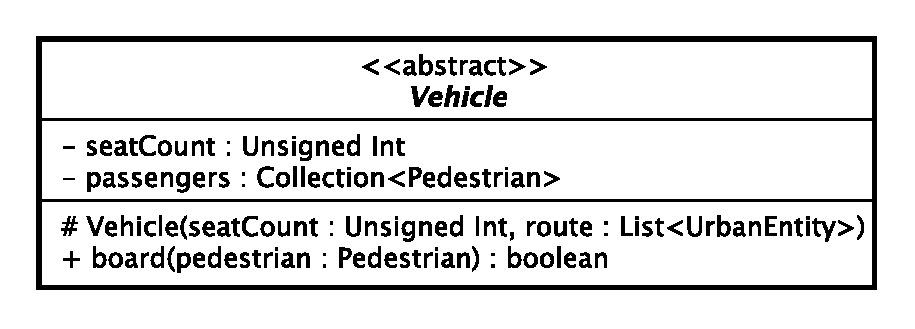
\includegraphics[scale=0.6,keepaspectratio]{images/solution/vehicle.eps}
\caption{App::Active::Vehicle}
\label{fig:sd-app-vehicle}
\end{figure}
\begin{itemize}
  \item \textbf{Description} \\
    It represents an entity that moves through the city carrying one or more
pedestrians.
  \item \textbf{Attribute}
  \begin{itemize}
    \item \texttt{- maxSeats: Unsigned Int} \\
The maximum number of seats in the vehicle.
    \item \texttt{- seat: ArrayList<Pedestrian>} \\
The list of passengers carried by the vehicle.
  \end{itemize}
  \item \textbf{Operation}
  \begin{itemize} 
    \item \texttt{+ Vehicle(maxSeats: Unsigned Int)} \\
Creates a vehicle specifying its maximum number of seats.
    \item \texttt{+ board(passenger: Pedestrian) : boolean} \\
If the vehicle is not full the pedestrian become a passenger and the method 
returns \textit{true}. Otherwise the access to the vehicle is not granted and 
the method returns false.
  \end{itemize}
\end{itemize}

\subsubsubsubsection{ConcreteVehicle}
\begin{figure}[h]
\centering
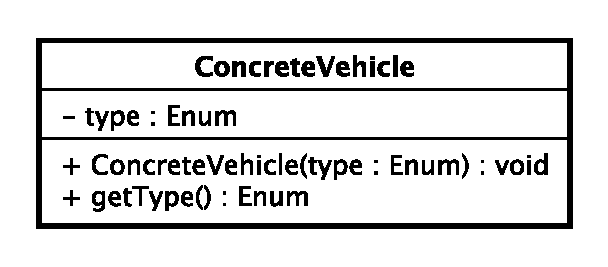
\includegraphics[scale=0.6,keepaspectratio]{images/solution/concrete_vehicle.eps}
\caption{App::Active::ConcreteVehicle}
\label{fig:sd-app-concrete-vehicle}
\end{figure}
\FloatBarrier
\begin{itemize}
  \item \textbf{Description} \\
It represents an entity that moves only on roadways.
  \item \textbf{Attribute}
  \begin{itemize}
    \item \texttt{- type: Enum} \\
Each vehicle has a type \{ car, motorcycle, sidecar \}.
  \end{itemize}
  \item \textbf{Operation}
  \begin{itemize} 
    \item \texttt{+ ConcreteVehicle(type: Enum)} \\
Creates a vehicle specifying its type.
    \item \texttt{+ getType() : Enum} \\
Returns the type of the concrete vehicle.
  \end{itemize}
\end{itemize} 

\subsubsubsubsection{Bicycle}
\begin{figure}[h]
\centering

\includegraphics[scale=0.6,keepaspectratio]{images/solution/bicycle.eps}
\caption{App::Active::Bicycle}
\label{fig:sd-app-bicycle}
\end{figure}
\FloatBarrier
\begin{itemize}
  \item \textbf{Description} \\
It represents an entity that moves only on bikepaths.
\end{itemize} 

\subsubsubsubsection{Bus}
\begin{figure}[h]
\centering

\includegraphics[scale=0.6,keepaspectratio]{images/solution/bus.eps}
\caption{App::Active::Bus}
\label{fig:sd-app-bus}
\end{figure}
\FloatBarrier
\begin{itemize}
  \item \textbf{Description} \\
It represents an entity that moves only on roadways and stops at each bus stop to
wait for passengers.
\end{itemize} 

\subsubsubsubsection{Pedestrian}
\begin{figure}[h]
\centering
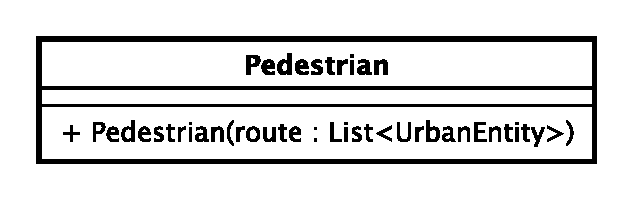
\includegraphics[scale=0.6,keepaspectratio]{images/solution/pedestrian.eps}
\caption{App::Active::Pedestrian}
\label{fig:sd-app-pedestrian}
\end{figure}
\begin{itemize}
  \item \textbf{Description} \\
It represents an entity that only moves on sidewalks.
\end{itemize} 

\subsubsubsubsection{Traffic Light}
\begin{figure}[h]
\centering
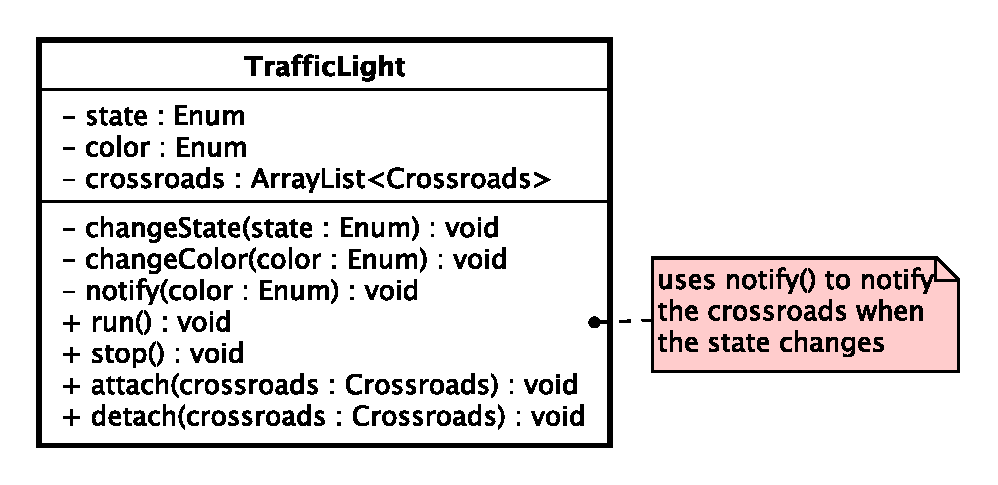
\includegraphics[scale=0.6,keepaspectratio]{images/solution/traffic_light.eps}
\caption{App::Active::TrafficLight}
\label{fig:sd-app-traffic-light}
\end{figure}
\FloatBarrier
\begin{itemize}
  \item \textbf{Description} \\
    It represents an entity that has two possible colors (green, red) and switch
between them after a specified period of time.
  \item \textbf{Attribute}
  \begin{itemize}
    \item \texttt{- state: Enum} \\
The possible states of the entity \{ running, stopped \}.
    \item \texttt{- color: Enum} \\
The possible colors of the entity \{ green, red \}.
  \end{itemize}
  \item \textbf{Operation}
  \begin{itemize} 
    \item \texttt{- changeState(state: Enum)} \\
Change the entity state. This method is used internally by public methods to 
change the entity behaviour.
    \item \texttt{- changeColor(color: Enum)} \\
Change the entity color. This method is used internally by public methods to 
switch between entity colors.
    \item \texttt{+ run(crossroads: Crossroads)} \\
Activates the entity which sets its state to \textit{running}. If its color is 
\textit{green} then it notifies the crossroads and then changes its color, 
otherwise it changes its color to \textit{green} and then notifies 
the crossroad. After changing its color it waits for n seconds.    
    \item \texttt{+ stop()} \\
Stops the entity which sets its state to \textit{stopped}.
  \end{itemize}
\end{itemize}

\subsubsubsection{ReactiveEntity}
\subsubsubsubsection{District}
\begin{figure}[h]
\centering
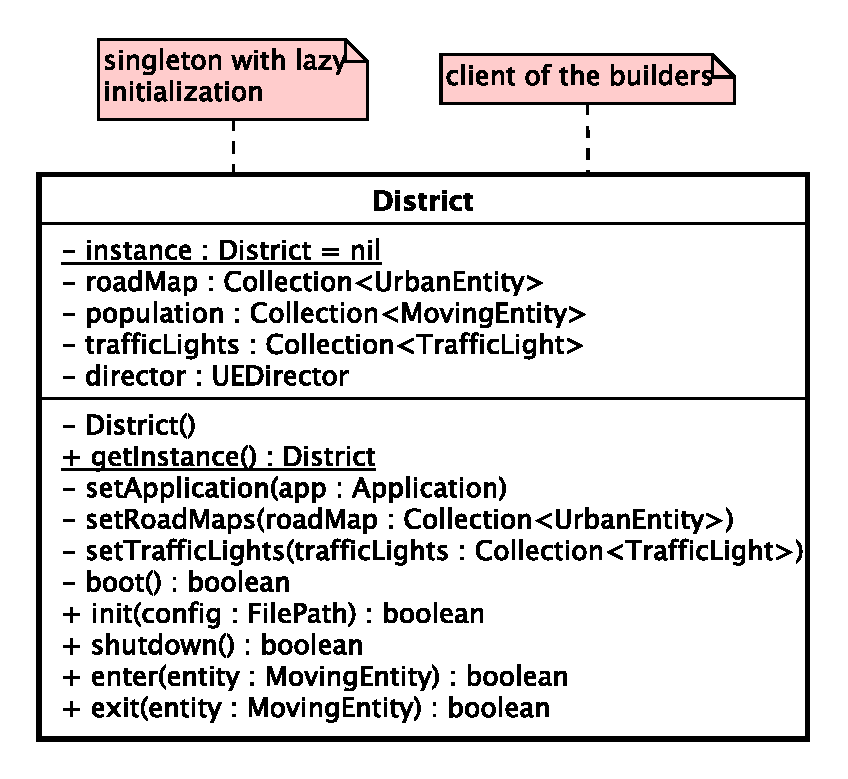
\includegraphics[scale=0.6,keepaspectratio]{images/solution/district.eps}
\caption{App::Reactive::District}
\label{fig:sd-app-district}
\end{figure}
\FloatBarrier
\begin{itemize}
  \item \textbf{Description} \\
It represents the master entity of the application layer. 
It has the responsibility to boot and shutdown the application layer.
  \item \textbf{Attribute}
  \begin{itemize}
    \item \texttt{- app: Application} \\
A reference to the interface of the application layer.
    \item \texttt{- roadMap: ArrayList<UrbanEntity>} \\
The urban entities of the district\footnote{Note that the name 
\textit{district} is only a convetion, indeed it is possible to have a 
real district splitted into different logical nodes of the system}
(i.e. crossroads and streets). 
    \item \texttt{- population: ArrayList<MovingEntity>} \\
The moving entities that reside on the district.
    \item \texttt{- trafficLight: ArrayList<TrafficLight>} \\
The traffic lights of the district.
    \item \texttt{- director: UEDirector} \\ 
The director of the city building process.
  \end{itemize}
  \item \textbf{Operation}
  \begin{itemize} 
    \item \texttt{- boot() : boolean} \\
Boots the application layer running all the active entities of the 
district (moving entities and traffic lights).
Returns true if the process completes neatly, false otherwise. 
This method is internally used by init.
    \item \texttt{+ init(config: FilePath) : boolean} \\
Creates and boots all the entities of the district according to the 
configuration file. Attaches each crossroads to the relative traffic light
if specified so in the configuration file. 
Returns true if the process completes neatly, false otherwise.
    \item \texttt{+ shutdown() : boolean} \\
Terminates the district. Returns true if the process completes neatly,
false otherwise.
    \item \texttt{+ enter(entity: MovingEntity) : boolean} \\
Notifies the district to add a new moving entity to the population.
Returns true if the process completes neatly, false otherwise.
    \item \texttt{+ exit(entity: MovingEntity) : boolean} \\
Notifies the district to pass a moving entity from the roadMap to the 
application layer interface which communicates to the middleware layer.
Returns true if the process completes neatly, false otherwise.
  \end{itemize}
\end{itemize} 

\subsubsubsubsection{UEDirector}
\begin{figure}[h]
\centering
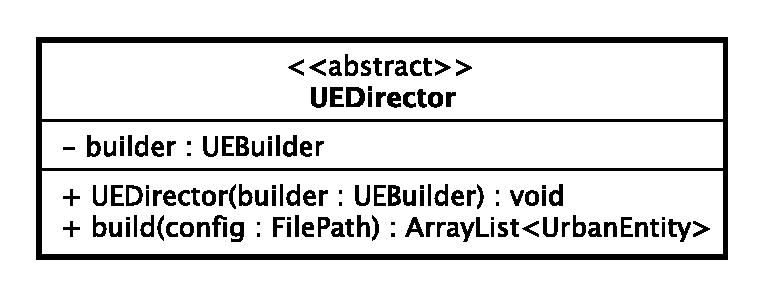
\includegraphics[scale=0.6,keepaspectratio]{images/solution/uedirector.eps}
\caption{App::Reactive::UEDirector}
\label{fig:sd-app-uedirector}
\end{figure}
\FloatBarrier
\begin{itemize}
  \item \textbf{Description} \\
    It represents the urban entity director which instructs the builder.
  \item \textbf{Attribute}
  \begin{itemize}
    \item \texttt{- builder: UEBuilder} \\
The builder object which builds parts of the district.
  \end{itemize}
  \item \textbf{Operation}
  \begin{itemize} 
    \item \texttt{+ UEDirector(builder: UEBuilder)} \\
Creates a director with its own builder object.
    \item \texttt{+ build(config: FilePath) : ArrayList<UrbanEntity>} \\
Builds a list of urban entities according to the configuration file. It uses the
builder multiple times to create incrementally a specific configuration of the
requested urban entity specified in the configuration file. 
  \end{itemize}
\end{itemize}

\subsubsubsubsection{Crossroads Director}
\begin{figure}[h]
\centering
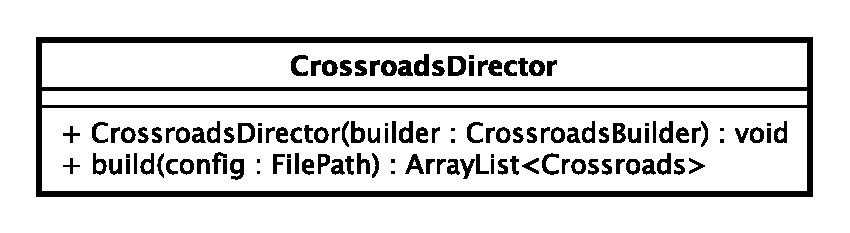
\includegraphics[scale=0.6,keepaspectratio]{images/solution/crossroads_director.eps}
\caption{App::Reactive::Crossroads Director}
\label{fig:sd-app-crossroads_director}
\end{figure}
\FloatBarrier
\begin{itemize}
  \item \textbf{Description} \\
    It represents the concrete director of the crossroads builder.
  \item \textbf{Operation}
  \begin{itemize} 
    \item \texttt{+ CrossroadsDirector(builder: CrossroadsBuilder)} \\
Creates a concrete crossroads director with its own crossroads builder.
    \item \texttt{+ build(config: FilePath) : ArrayList<Crossroads>} \\
Builds a list of crossroads according to the configuration file. 
It uses the builder multiple times 
to create incrementally a configuration of the requested crossroads as specified
in the configuration file. 
  \end{itemize}
\end{itemize}

\subsubsubsubsection{Street Director}
\begin{figure}[h]
\centering
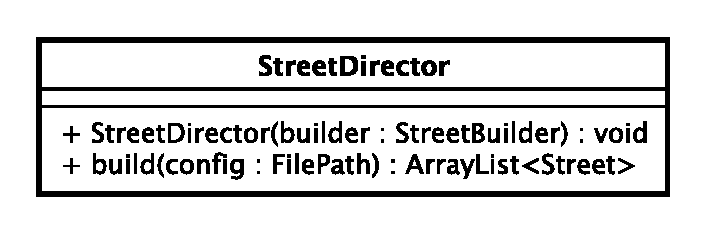
\includegraphics[scale=0.6,keepaspectratio]{images/solution/street_director.eps}
\caption{App::Reactive::Street Director}
\label{fig:sd-app-street_director}
\end{figure}
\FloatBarrier
\begin{itemize}
  \item \textbf{Description} \\
    It represents the concrete director of the street builder.
  \item \textbf{Operation}
  \begin{itemize} 
    \item \texttt{+ StreetDirector(builder: StreetBuilder)} \\
Creates a concrete street director with its own street builder.
    \item \texttt{+ build(config: FilePath) : ArrayList<Street>} \\
Builds a list of streets according to the configuration file. 
It uses the builder multiple times to create incrementally a 
specific configuration of the requested street specified 
in the configuration file. 
  \end{itemize}
\end{itemize}

\subsubsubsubsection{UEBuilder}
\begin{figure}[h]
\centering
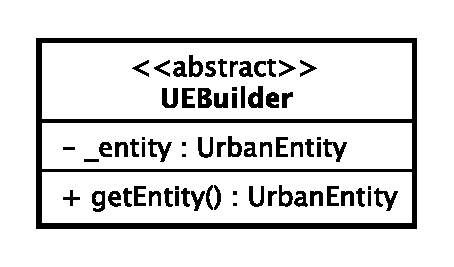
\includegraphics[scale=0.6,keepaspectratio]{images/solution/uebuilder.eps}
\caption{App::Reactive::UEBuilder}
\label{fig:sd-app-uebuilder}
\end{figure}
\FloatBarrier
\begin{itemize}
  \item \textbf{Description} \\
    It represents an entity that moves through the city carrying one or more
pedestrians.
  \item \textbf{Attribute}
  \begin{itemize}
    \item \texttt{- \_entity: UrbanEntity} \\
The entity which the builder incrementally constructs.
  \end{itemize}
  \item \textbf{Operation}
  \begin{itemize} 
    \item \texttt{+ getEntity() : UrbanEntity} \\
Returns the final product of the building.
  \end{itemize}
\end{itemize}

\subsubsubsubsection{CrossroadsBuilder}
\begin{figure}[h]
\centering
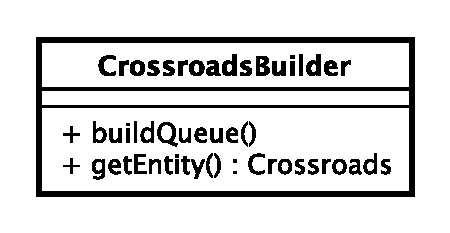
\includegraphics[scale=0.6,keepaspectratio]{images/solution/crossroads_builder.eps}
\caption{App::Reactive::CrossroadsBuilder}
\label{fig:sd-app-crossroads_builder}
\end{figure}
\FloatBarrier
\begin{itemize}
  \item \textbf{Description} \\
    It represents the builder of crossroads entities. 
  \item \textbf{Operation}
  \begin{itemize} 
    \item \texttt{+ buildTrafficLight()} \\
Adds a new traffic light to the crossroads.
    \item \texttt{+ buildQueue()} \\
Adds a new queue of moving entities to the crossroads.
    \item \texttt{+ getEntity() : Crossroads} \\
Returns the crossroads.
  \end{itemize}
\end{itemize}

\subsubsubsubsection{StreetBuilder}
\begin{figure}[h]
\centering
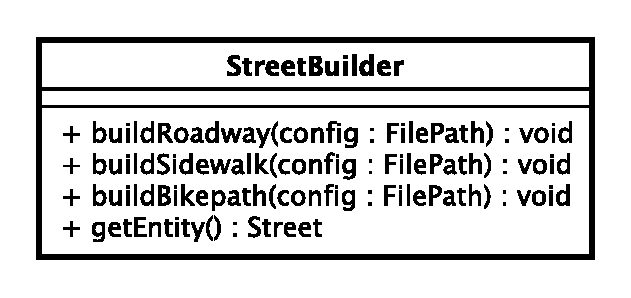
\includegraphics[scale=0.6,keepaspectratio]{images/solution/street_builder.eps}
\caption{App::Reactive::StreetBuilder}
\label{fig:sd-app-street_builder}
\end{figure}
\FloatBarrier
\begin{itemize}
  \item \textbf{Description} \\
    It represents the builder of street entities. 
  \item \textbf{Operation}
  \begin{itemize} 
    \item \texttt{+ buildRoadway(config: FilePath)} \\
Builds a roadway using roadwayfactory according to a specific configuration.
    \item \texttt{+ buildSidewalk(config: FilePath)} \\
Builds a sidewalk using sidewalkfactory according to a specific configuration.
    \item \texttt{+ buildBikepath(config: FilePath)} \\
Builds a bikepath using bikepathfactory according to a specific configuration.
    \item \texttt{+ getEntity() : Street} \\
Returns the street.
  \end{itemize}
\end{itemize}

\subsubsubsubsection{Urban Entity}
\begin{figure}[h]
\centering
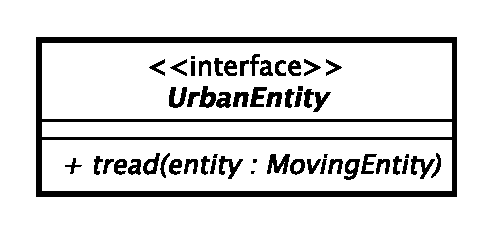
\includegraphics[scale=0.6,keepaspectratio]{images/solution/urban_entity.eps}
\caption{App::Reactive::Urban Entity}
\label{fig:sd-app-urban-entity}
\end{figure}
\FloatBarrier
\begin{itemize}
  \item \textbf{Description} \\
    It represents one of the entities the district infrastructure is composed
    of.
  \item \textbf{Operation}
  \begin{itemize} 
    \item \texttt{\textit{+ tread(entity: MovingEntity)}} \\
    Abstract method through which the urban infrastructure can be treaded by a
    moving entity.
  \end{itemize}
\end{itemize}

\subsubsubsubsection{Crossroads}
\begin{figure}[h]
\centering
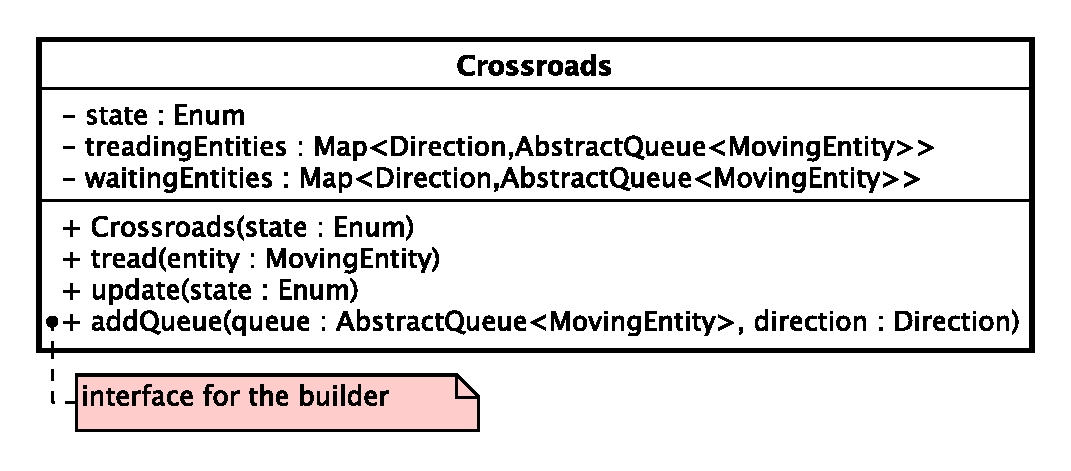
\includegraphics[scale=0.6,keepaspectratio]{images/solution/crossroads.eps}
\caption{App::Reactive::Crossroads}
\label{fig:sd-app-crossroads}
\end{figure}
\FloatBarrier
\begin{itemize}
  \item \textbf{Description} \\
    It represents a concrete crossroads entity. It is a protected object.
  \item \textbf{Attribute}
  \begin{itemize}
    \item \texttt{- state: Enum} \\
The traffic light state indicates which directions to free.
    \item \texttt{- treading: Map<Direction, AbstractQueue<MovingEntity>>} \\
The queue of moving entities which are treading the crossroads.
    \item \texttt{- waiting: Map<Direction, AbstratQueue<MovingEntity>>} \\
The queue of moving entities which are waiting to tread the crossroads. 
  \item \textbf{Operation}
  \begin{itemize} 
    \item \texttt{+ tread(entity: MovingEntity)} \\
Implements the treading of the crossroads.
    \item \texttt{+ update(state: Enum)} \\
Updates the state value of the crossroads.
    \item \texttt{+ addQueue(queue: AbstratQueue<MovingEntity>, direction: Direction)} \\
Add a new queue to waiting and treading maps with the specified direction.
  \end{itemize}
\end{itemize}

\subsubsubsubsection{Direction}
\begin{figure}[h]
\centering
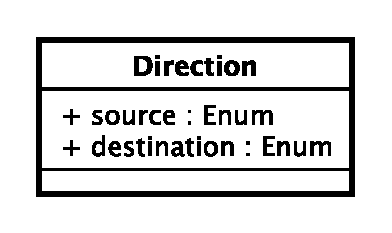
\includegraphics[scale=0.6,keepaspectratio]{images/solution/direction.eps}
\caption{App::Reactive::Direction}
\label{fig:sd-app-direction}
\end{figure}
\FloatBarrier
\begin{itemize}
  \item \textbf{Description} \\
    It represents the direction. 
  \item \textbf{Attribute}
  \begin{itemize}
    \item \texttt{- source: Enum} \\
The source from which an entity arrives. It has four possible
values \{ north, south, east, west \}
    \item \texttt{- destination: Enum} \\
The destination where the entity is directed. It has the same possible
values of source.
  \end{itemize}
\end{itemize}

\subsubsubsubsection{Street Factory}
\begin{figure}[h]
\centering
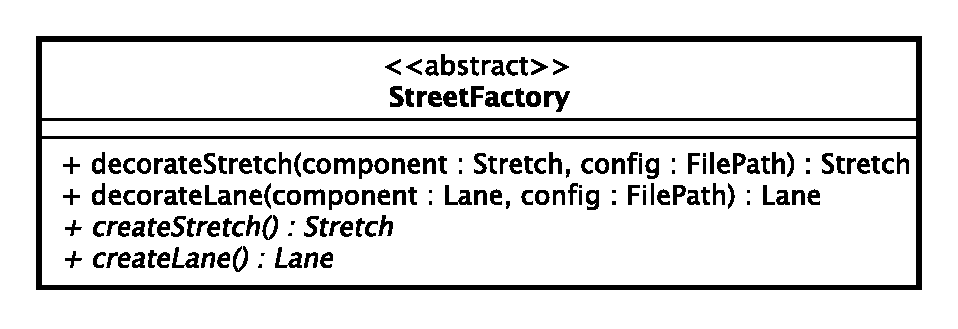
\includegraphics[scale=0.6,keepaspectratio]{images/solution/street_factory.eps}
\caption{App::Reactive::StreetFactory}
\label{fig:sd-app-street-factory}
\end{figure}
\FloatBarrier
\begin{itemize}
  \item \textbf{Description} \\
    It represents the base class of the abstract factory pattern. The 
not abstract methods of this class are used by StreetBuilder during the
building phase.
  \item \textbf{Operation} \\
  \begin{itemize} 
    \item \texttt{+ decorateStretch(component: Stretch, config: FilePath)} \\
Decorates an existing stretch component according to the configuration file parameters.
    \item \texttt{+ decorateLane(component: Lane, config: FilePath)} \\
Decorates an existing lane component according to the configuration file parameters.
    \item \texttt{\textit{+ createStretch() : Stretch}} \\
Abstract method which will create a new stretch component.
    \item \texttt{\textit{+ createLane() : Lane}} \\
Abstract method which will create a new lane component.
  \end{itemize}
\end{itemize}

\subsubsubsubsection{Roadway Factory}
\begin{figure}[h]
\centering
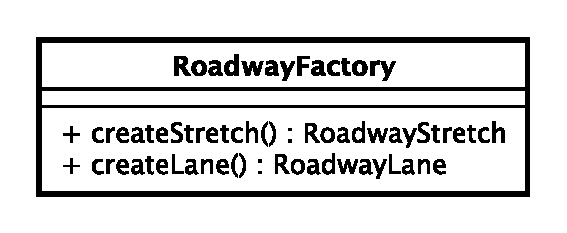
\includegraphics[scale=0.6,keepaspectratio]{images/solution/roadway_factory.eps}
\caption{App::Reactive::RoadwayFactory}
\label{fig:sd-app-roadway-factory}
\end{figure}
\FloatBarrier
\begin{itemize}
  \item \textbf{Description} \\
It represents a factory which creates roadway components.
  \item \textbf{Operation} \\
  \begin{itemize} 
    \item \texttt{+ createStretch() : RoadwayStretch} \\
Creates a new roadway stretch component.
    \item \texttt{+ createLane() : RoadwayLane} \\
Creates a new roadway lane component.
  \end{itemize}
\end{itemize}

\subsubsubsubsection{Sidewalk Factory}
\begin{figure}[h]
\centering
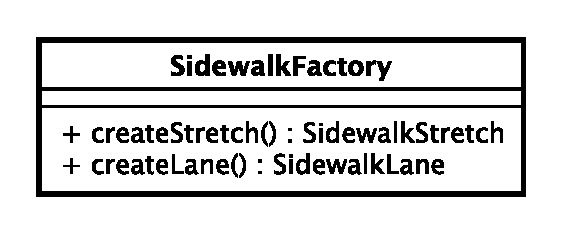
\includegraphics[scale=0.6,keepaspectratio]{images/solution/sidewalk_factory.eps}
\caption{App::Reactive::SidewalkFactory}
\label{fig:sd-app-sidewalk-factory}
\end{figure}
\FloatBarrier
\begin{itemize}
  \item \textbf{Description} \\
It represents a factory which creates sidewalk components.
  \item \textbf{Operation} \\
  \begin{itemize} 
    \item \texttt{+ createStretch() : SidewalkStretch} \\
Creates a new sidewalk stretch component.
    \item \texttt{+ createLane() : SidewalkLane} \\
Creates a new sidewalk lane component.
  \end{itemize}
\end{itemize}

\subsubsubsubsection{Bikepath Factory}
\begin{figure}[h]
\centering
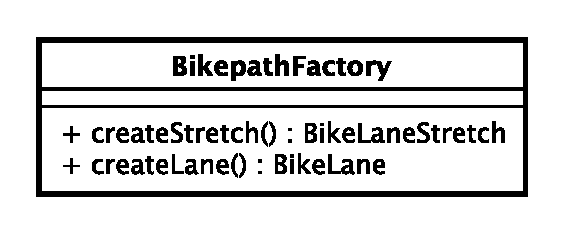
\includegraphics[scale=0.6,keepaspectratio]{images/solution/bikepath_factory.eps}
\caption{App::Reactive::BikepathFactory}
\label{fig:sd-app-bikepath-factory}
\end{figure}
\FloatBarrier
\begin{itemize}
  \item \textbf{Description} \\
It represents a factory which creates bikepath components.
  \item \textbf{Operation} \\
  \begin{itemize} 
    \item \texttt{+ createStretch() : BikeLaneStretch} \\
Creates a new bike lane stretch component.
    \item \texttt{+ createLane() : BikeLane} \\
Creates a new bike lane component.
  \end{itemize}
\end{itemize}

\subsubsubsubsection{Street}
\begin{figure}[h]
\centering
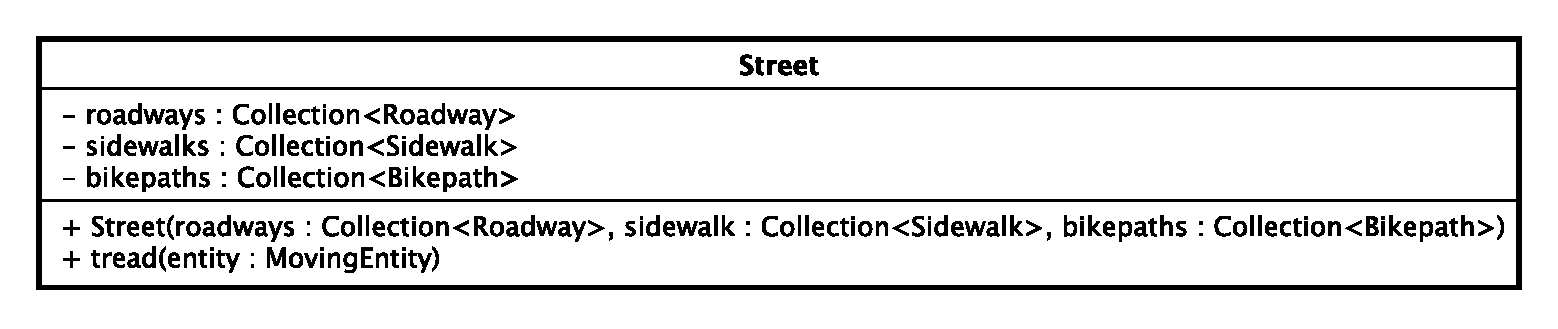
\includegraphics[scale=0.6,keepaspectratio]{images/solution/street.eps}
\caption{App::Reactive::Street}
\label{fig:sd-app-street}
\end{figure}
\FloatBarrier
\begin{itemize}
  \item \textbf{Description} \\
    It represents a concrete street.
  \item \textbf{Attribute}
  \begin{itemize}
    \item \texttt{- roadway: ArrayList<Roadway>} \\
A street has a roadway.
    \item \texttt{- sidewalk: ArrayList<Sidewalk>} \\
A street can have one or more sidewalks (typically one for each side
of the street).
    \item \texttt{- bikepath: ArrayList<Bikepath>} \\
A street can have one or more bikepaths, (typically one for each side
of the street).
  \end{itemize}
  \item \textbf{Operation}
  \begin{itemize} 
    \item \texttt{+ tread(entity: MovingEntity)} \\
Moves the entity in the proper part of the street based on the
concrete type of the entity (i.e. pedestrians will move on sidewalks).
  \end{itemize}
\end{itemize}

\subsubsubsubsection{Roadway}
\begin{figure}[h]
\centering
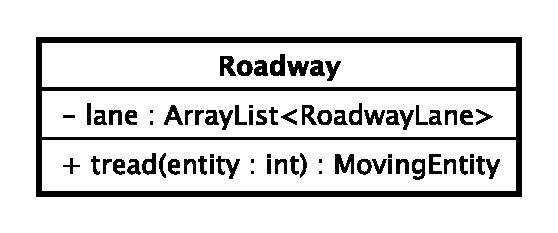
\includegraphics[scale=0.6,keepaspectratio]{images/solution/roadway.eps}
\caption{App::Reactive::Roadway}
\label{fig:sd-app-roadway}
\end{figure}
\FloatBarrier
\begin{itemize}
  \item \textbf{Description} \\
    It represents a concrete roadway which is composed of one or more lanes.
  \item \textbf{Attribute}
  \begin{itemize}
    \item \texttt{- lane: ArrayList<RoadwayLane>} \\
A roadway is composed of lanes.
  \end{itemize}
  \item \textbf{Operation}
  \begin{itemize} 
    \item \texttt{+ tread(entity: MovingEntity)} \\
Moves the entity on the correct lane based on the current entity route. 
  \end{itemize}
\end{itemize}

\subsubsubsubsection{Bikepath}
\begin{figure}[h]
\centering
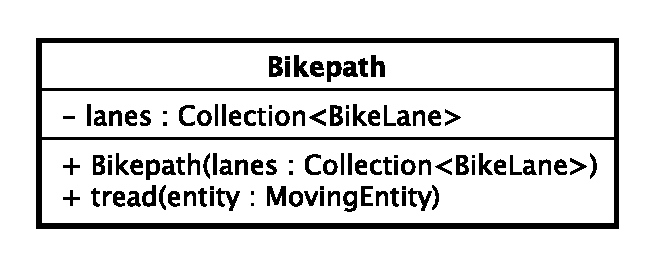
\includegraphics[scale=0.6,keepaspectratio]{images/solution/bikepath.eps}
\caption{App::Reactive::Bikepath}
\label{fig:sd-app-bikepath}
\end{figure}
\FloatBarrier
\begin{itemize}
  \item \textbf{Description} \\
    It represents a concrete bikepath which is composed by at least one lane.
  \item \textbf{Attribute}
  \begin{itemize}
    \item \texttt{- lane: ArrayList<BikeLane>} \\
A bikepath is composed by lanes.
  \end{itemize}
  \item \textbf{Operation}
  \begin{itemize} 
    \item \texttt{+ tread(entity: MovingEntity)} \\
Moves the entity on the correct lane based on the current entity route. 
  \end{itemize}
\end{itemize}

\subsubsubsubsection{Sidewalk}
\begin{figure}[h]
\centering
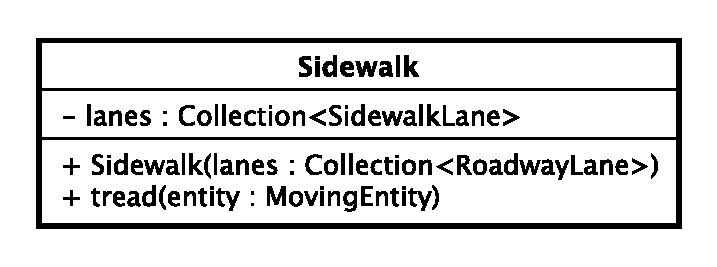
\includegraphics[scale=0.6,keepaspectratio]{images/solution/sidewalk.eps}
\caption{App::Reactive::Sidewalk}
\label{fig:sd-app-sidewalk}
\end{figure}
\FloatBarrier
\begin{itemize}
  \item \textbf{Description} \\
    It represents a concrete sidewalk which is composed by at least one lane.
  \item \textbf{Attribute}
  \begin{itemize}
    \item \texttt{- lane: ArrayList<SidewalkLane>} \\
A sidewalk is composed by lanes.
  \end{itemize}
  \item \textbf{Operation}
  \begin{itemize} 
    \item \texttt{+ tread(entity: MovingEntity)} \\
Moves the entity on the correct lane based on the current entity route. 
  \end{itemize}
\end{itemize}

\subsubsubsubsection{Lane}
\begin{figure}[h]
\centering
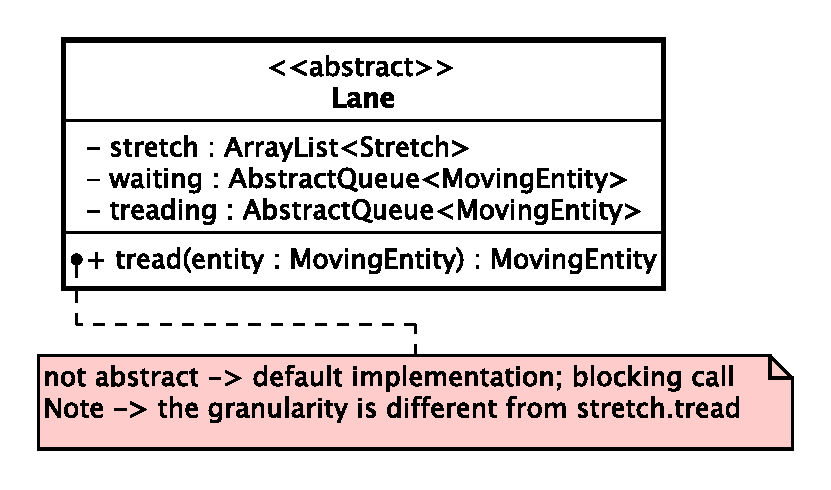
\includegraphics[scale=0.6,keepaspectratio]{images/solution/lane.eps}
\caption{App::Reactive::Lane}
\label{fig:sd-app-lane}
\end{figure}
\FloatBarrier
\begin{itemize}
  \item \textbf{Description} \\
    It represents a lane entity. It is a protected object composed of one or
    more stretches.
  \item \textbf{Attribute}
  \begin{itemize}
    \item \texttt{- size: Unsigned Int} \\
The size of the stretch/treading queue.
    \item \texttt{- stretch: ArrayList<Stretch>} \\
The list of stretches which compose the lane.
    \item \texttt{- treading: AbstractQueue<MovingEntity>} \\
The queue of moving entities which are treading the lane.
    \item \texttt{- waiting: AbstractQueue<MovingEntity>} \\
The queue of moving entities which are waiting to tread the lane. 
  \end{itemize}
  \item \textbf{Operation}
  \begin{itemize} 
    \item \texttt{+ Lane(size: Unsigned Int, stretch: ArrayList<Stretch>)} \\
Creates a \texttt{Lane} object with a specific size and list of stretches.
    \item \texttt{+ tread(entity: MovingEntity)} \\
Implements the lane treading. Moves the entity on the stretches which are 
in the moving entity route.
  \end{itemize}
\end{itemize}

\subsubsubsubsection{Stretch}
\begin{figure}[h]
\centering
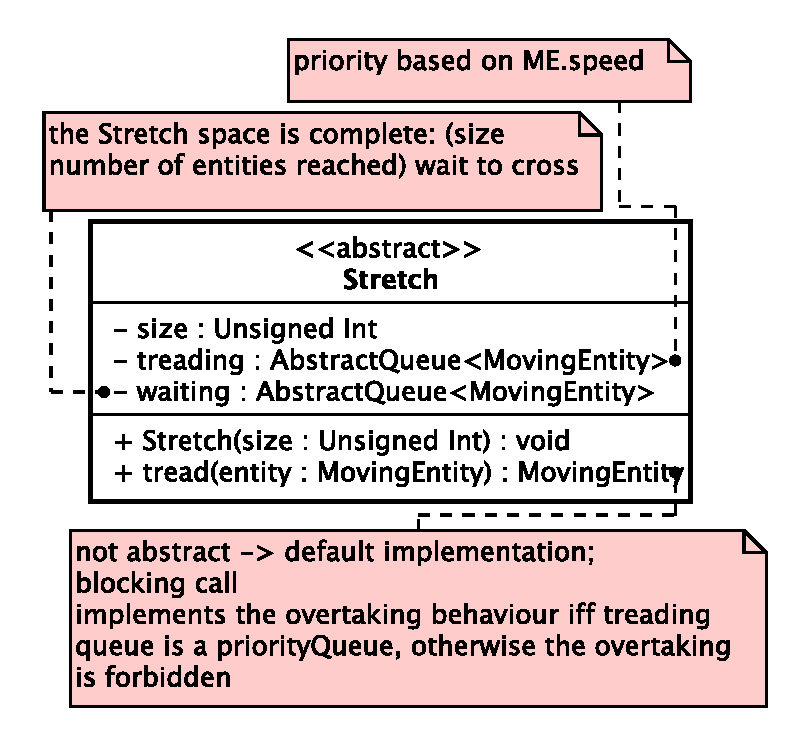
\includegraphics[scale=0.6,keepaspectratio]{images/solution/stretch.eps}
\caption{App::Reactive::Stretch}
\label{fig:sd-app-stretch}
\end{figure}
\FloatBarrier
\begin{itemize}
  \item \textbf{Description} \\
    It represents a stretch entity. It is a protected object.
  \item \textbf{Attribute}
  \begin{itemize}
    \item \texttt{- size: Unsigned Int} \\
The size of the stretch/treading queue.
    \item \texttt{- treading: AbstractQueue<MovingEntity>} \\
The queue of moving entities which are treading the stretch. If the concrete type
is PriorityQueue then the stretch allows the overtaking between the moving entities.
This is implemented through a priority queue ordered by decresing speed.
    \item \texttt{- waiting: AbstractQueue<MovingEntity>} \\
The queue of moving entities which are waiting to tread the stretch. 
  \end{itemize}
  \item \textbf{Operation}
  \begin{itemize}
    \item \texttt{+ Stretch(size: Unsigned Int)} \\
Creates a stretch object with a specific size.
    \item \texttt{+ tread(entity: MovingEntity)} \\
Implements the treading of the stretch. The current speed of the moving entity
is calculated first, then the entity is placed in a treading queue which has a  
timeout, after the deadline elapsed the queue is flushed and the entity can proceed
along their route.
  \end{itemize}
\end{itemize}

\subsubsubsubsection{Roadway Stretch}
\begin{figure}[h]
\centering
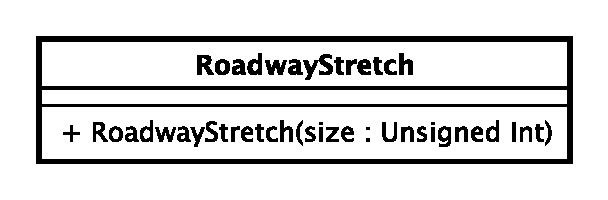
\includegraphics[scale=0.6,keepaspectratio]{images/solution/roadway_stretch.eps}
\caption{App::Reactive::RoadwayStretch}
\label{fig:sd-app-roadway_stretch}
\end{figure}
\FloatBarrier
\begin{itemize}
  \item \textbf{Description} \\
    It represents a roadway stretch entity. It is a protected object. Only specific types of vehicles can tread this kind of stretch.
\end{itemize}

\subsubsubsubsection{Bike Lane Stretch}
\begin{figure}[h]
\centering

\includegraphics[scale=0.6,keepaspectratio]{images/solution/bikelane_stretch.eps}
\caption{App::Reactive::BikeLaneStretch}
\label{fig:sd-app-bikelane_stretch}
\end{figure}
\FloatBarrier
\begin{itemize}
  \item \textbf{Description} \\
    It represents a bike lane stretch entity. It is a protected object. Only bycicles 
can tread this kind of stretch.
\end{itemize}

\subsubsubsubsection{Sidewalk Stretch}
\begin{figure}[h]
\centering
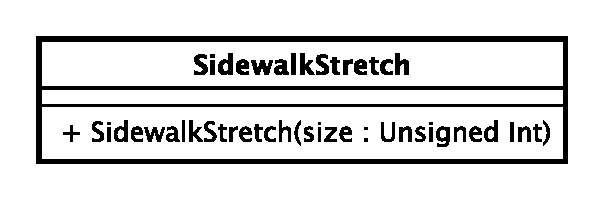
\includegraphics[scale=0.6,keepaspectratio]{images/solution/sidewalk_stretch.eps}
\caption{App::Reactive::SidewalkStretch}
\label{fig:sd-app-sidewalk_stretch}
\end{figure}
\FloatBarrier
\begin{itemize}
  \item \textbf{Description} \\
    It represents a sidewalk stretch entity. It is a protected object. Only pedestrians
can tread this kind of stretch.
\end{itemize}

\subsubsubsection{PassiveEntity}

